%%%%%%%%%%%%%%%%%%%%%%%%%%%%%%%%%%%%%%%%%%%%%%%%%%%%%%%%%%%%%%%%%%%%%%%%%%%%%%%%
%%%%%%%%%%%%%%%%%%%%%%%%%%%%%%%%%%%%%%%%%%%%%%%%%%%%%%%%%%%%%%%%%%%%%%%%%%%%%%%%
%%                                                                            %%
%% thesistemplate.tex version 3.20 (2018/08/31)                               %%
%% The LaTeX template file to be used with the aaltothesis.sty (version 3.20) %%
%% style file.                                                                %%
%% This package requires pdfx.sty v. 1.5.84 (2017/05/18) or newer.            %%
%%                                                                            %%
%% This is licensed under the terms of the MIT license below.                 %%
%%                                                                            %%
%% Written by Luis R.J. Costa.                                                %%
%% Currently developed at the Learning Services of Aalto University School of %%
%% Electrical Engineering by Luis R.J. Costa since May 2017.                  %%
%%                                                                            %%
%% Copyright 2017-2018, by Luis R.J. Costa, luis.costa@aalto.fi,              %%
%% Copyright 2017-2018 Swedish translations in aaltothesis.cls by Elisabeth   %%
%% Nyberg, elisabeth.nyberg@aalto.fi and Henrik Wallén,                       %%
%% henrik.wallén@aalto.fi.                                                    %%
%% Copyright 2017-2018 Finnish documentation in the template opinnaytepohja.tex%%
%% by Perttu Puska, perttu.puska@aalto.fi, and Luis R.J. Costa.               %%
%% Copyright 2018 English template thesistemplate.tex by Luis R.J. Costa.     %%
%% Copyright 2018 Swedish template kandidatarbetsbotten.tex by Henrik Wallén. %%
%%                                                                            %%
%% Permission is hereby granted, free of charge, to any person obtaining a    %%
%% copy of this software and associated documentation files (the "Software"), %%
%% to deal in the Software without restriction, including without limitation  %%
%% the rights to use, copy, modify, merge, publish, distribute, sublicense,   %%
%% and/or sell copies of the Software, and to permit persons to whom the      %%
%% Software is furnished to do so, subject to the following conditions:       %%
%% The above copyright notice and this permission notice shall be included in %%
%% all copies or substantial portions of the Software.                        %%
%% THE SOFTWARE IS PROVIDED "AS IS", WITHOUT WARRANTY OF ANY KIND, EXPRESS OR %%
%% IMPLIED, INCLUDING BUT NOT LIMITED TO THE WARRANTIES OF MERCHANTABILITY,   %%
%% FITNESS FOR A PARTICULAR PURPOSE AND NONINFRINGEMENT. IN NO EVENT SHALL    %%
%% THE AUTHORS OR COPYRIGHT HOLDERS BE LIABLE FOR ANY CLAIM, DAMAGES OR OTHER %%
%% LIABILITY, WHETHER IN AN ACTION OF CONTRACT, TORT OR OTHERWISE, ARISING    %%
%% FROM, OUT OF OR IN CONNECTION WITH THE SOFTWARE OR THE USE OR OTHER        %%
%% DEALINGS IN THE SOFTWARE.                                                  %%
%%                                                                            %%
%%                                                                            %%
%%%%%%%%%%%%%%%%%%%%%%%%%%%%%%%%%%%%%%%%%%%%%%%%%%%%%%%%%%%%%%%%%%%%%%%%%%%%%%%%
%%                                                                            %%
%%                                                                            %%
%% An example for writing your thesis using LaTeX                            %%
%% Original version and development work by Luis Costa, changes to the text   %% 
%% in the Finnish template by Perttu Puska.                                   %%
%% Support for Swedish added 15092014                                         %%
%% PDF/A-b support added on 15092017                                          %%
%% PDF/A-2 support added on 24042018                                          %%
%%                                                                            %%
%% This example consists of the files                                         %%
%%         thesistemplate.tex (version 3.20) (for text in English)            %%
%%         opinnaytepohja.tex (version 3.20) (for text in Finnish)            %%
%%         kandidatarbetsbotten.tex (version 1.00) (for text in Swedish)      %%
%%         aaltothesis.cls (version 3.20)                                      %%
%%         kuva1.eps (graphics file)                                          %%
%%         kuva2.eps (graphics file)                                          %%
%%         kuva1.jpg (graphics file)                                          %%
%%         kuva2.jpg (graphics file)                                          %%
%%         kuva1.png (graphics file)                                          %%
%%         kuva2.png (graphics file)                                          %%
%%         kuva1.pdf (graphics file)                                          %%
%%         kuva2.pdf (graphics file)                                          %%
%%                                                                            %%
%%                                                                            %%
%% Typeset in Linux either with                                               %%
%% pdflatex: (recommended method)                                             %%
%%             $ pdflatex thesistemplate                                      %%
%%             $ pdflatex thesistemplate                                      %%
%%                                                                            %%
%%   The result is the file thesistemplate.pdf that is PDF/A compliant, if    %%
%%   you have chosen the proper \documenclass options (see comments below)    %%
%%   and your included graphics files have no problems.
%%                                                                            %%
%% Or                                                                         %%
%% latex: (this method is not recommended)                                    %%
%%             $ latex thesistemplate                                         %%
%%             $ latex thesistemplate                                         %%
%%                                                                            %%
%%   The result is the file thesistemplate.dvi, which is converted to ps      %%
%%   format as follows:                                                       %%
%%                                                                            %%
%%             $ dvips thesistemplate -o                                      %%
%%                                                                            %%
%%   and then to pdf as follows:                                              %%
%%                                                                            %%
%%             $ ps2pdf thesistemplate.ps                                     %%
%%                                                                            %%
%%   This pdf file is not PDF/A compliant. You must must make it so using,    %%
%%   e.g., Acrobat Pro or PDF-XChange.                                        %%
%%                                                                            %%
%%                                                                            %%
%% Explanatory comments in this example begin with the characters %%, and     %%
%% changes that the user can make with the character %                        %%
%%                                                                            %%
%%%%%%%%%%%%%%%%%%%%%%%%%%%%%%%%%%%%%%%%%%%%%%%%%%%%%%%%%%%%%%%%%%%%%%%%%%%%%%%%
%%%%%%%%%%%%%%%%%%%%%%%%%%%%%%%%%%%%%%%%%%%%%%%%%%%%%%%%%%%%%%%%%%%%%%%%%%%%%%%%
%%
%% WHAT is PDF/A
%%
%% PDF/A is the ISO-standardized version of the pdf. The standard's goal is to
%% ensure that he file is reproducible even after a long time. PDF/A differs
%% from pdf in that it allows only those pdf features that support long-term
%% archiving of a file. For example, PDF/A requires that all used fonts are
%% embedded in the file, whereas a normal pdf can contain only a link to the
%% fonts in the system of the reader of the file. PDF/A also requires, among
%% other things, data on colour definition and the encryption used.
%% Currently three PDF/A standards exist:
%% PDF/A-1: based on PDF 1.4, standard ISO19005-1, published in 2005.
%%          Includes all the requirements essential for long-term archiving.
%% PDF/A-2: based on PDF 1.7, standard ISO19005-2, published in 2011.
%%          In addition to the above, it supports embedding of OpenType fonts,
%%          transparency in the colour definition and digital signatures.
%% PDF/A-3: based on PDF 1.7, standard ISO19005-3, published in 2012.
%%          Differs from the above only in that it allows embedding of files in
%%          any format (e.g., xml, csv, cad, spreadsheet or word processing
%%          formats) into the pdf file.
%% PDF/A-1 files are not necessarily PDF/A-2 -compatible and PDF/A-2 are not
%% necessarily PDF/A-1 -compatible.
%% All of the above PDF/A standards have two levels:
%% b: (basic) requires that the visual appearance of the document is reliably
%%    reproducible.
%% a (accessible) in addition to the b-level requirements, specifies how
%%   accessible the pdf file is to assistive software, say, for the physically
%%   impaired.
%% For more details on PDF/A, see, e.g., https://en.wikipedia.org/wiki/PDF/A
%%
%%
%% WHICH PDF/A standard should my thesis conform to?
%%
%% Primarily to the PDF/A-1b standard. All the figures and graphs typically
%% use in thesis work do not require transparency features, a basic '2-D'
%% visualisation suffices. The font to be used are specified in this template
%% and they should not be changed. However, if you have figures where
%% transparency characteristics matter, use the PDF/A-2b standard. Do not use
%% the PDF/A-3b standard for your thesis.
%%
%%
%% WHAT graphics format can I use to produce my PDF/A compliant file?
%%
%% When using pdflatex to compile your work, use jpg, png or pdf files. You may
%% have PDF/A compliance problems with figures in pdf format. Do not use PDF/A
%% compliant graphics files.
%% If you decide to use latex to compile your work, the only acceptable file
%% format for your figure is eps. DO NOT use the ps format for your figures.

%% USE one of these:
%% * the first when using pdflatex, which directly typesets your document in the
%%   chosen pdf/a format and you want to publish your thesis online,

%% * the second when you want to print your thesis to bind it, or
%% * the third when producing a ps file and a pdf/a from it.
%%
\documentclass[english, 12pt, a4paper, sci, utf8, a-1b, online]{aaltothesis}
% \documentclass[english, 12pt, a4paper, sci, utf8, a-1b]{aaltothesis}
% \documentclass[english, 12pt, a4paper, sci, dvips, online]{aaltothesis}

%% Use the following options in the \documentclass macro above:
%% your school: arts, biz, chem, elec, eng, sci
%% the character encoding scheme used by your editor: utf8, latin1
%% thesis language: english, finnish, swedish
%% make an archive suitable PDF/A-1b or PDF/A-2b compliant file: a-1b, a-2b
%%                    (with pdflatex, a normal pdf containing metadata is
%%                     produced without the a-*b option)
%% typeset in symmetric layout and blue hypertext for online publication: online
%%            (no option is the default, resulting in a wide margin on the
%%             binding side of the page and black hypertext)
%% two-sided printing: twoside (default is one-sided printing)
%%

%% Use one of these if you write in Finnish (see the Finnish template
%% opinnaytepohja.tex)
%\documentclass[finnish, 12pt, a4paper, elec, utf8, a-1b, online]{aaltothesis}
%\documentclass[finnish, 12pt, a4paper, elec, utf8, a-1b]{aaltothesis}
%\documentclass[finnish, 12pt, a4paper, elec, dvips, online]{aaltothesis}

\usepackage{graphicx}
\usepackage{tabularx}
\usepackage{longtable}
\usepackage{float}
\usepackage{caption}
\usepackage{titlesec}
\usepackage{hyperref}
\usepackage{csquotes}

%% Math fonts, symbols, and formatting; these are usually needed
\usepackage{amsfonts,amssymb,amsbsy,amsmath}

% Different bibliography styles can be found from https://www.overleaf.com/learn/latex/Bibtex_bibliography_styles
% current bibliography style found from https://tex.stackexchange.com/questions/131518/help-with-citation-in-text-in-parentheses-etc-with-biblatex-apa
\usepackage[
backend=biber,
style=apa,
sortcites=true,
sorting=nyt
]{biblatex}
\addbibresource{thesis.bib}

%% Change the school field to specify your school if the automatically set name
%% is wrong
% \university{aalto-yliopisto}
% \school{Sähkötekniikan korkeakoulu}

%% Edit to conform to your degree programme
%%
\degreeprogram{Computer, Communication and Information Sciences}
%%

%% Your major
%%
\major{Software and Service Engineering}
%%

%% Major subject code
%%
\code{SCI3043}
%%
 
%% Choose one of the three below
%%
%\univdegree{BSc}
\univdegree{MSc}
%\univdegree{Lic}
%%

%% Your name (self explanatory...)
%%
\thesisauthor{Anders Nylund}
%%

%% Your thesis title comes here and possibly again together with the Finnish or
%% Swedish abstract. Do not hyphenate the title, and avoid writing too long a
%% title. Should LaTeX typeset a long title unsatisfactorily, you might have to
%% force a line break using the \\ control characters.
%% In this case...
%% Remember, the title should not be hyphenated!
%% A possible "and" in the title should not be the last word in the line, it
%% begins the next line.
%% Specify the title again without the line break characters in the optional
%% argument in box brackets. This is done because the title is part of the 
%% metadata in the pdf/a file, and the metadata cannot contain line breaks.
%%
\thesistitle{Developer Experience}
%\thesistitle[Title of the thesis]{Title of\\ the thesis}
%%

%%
\place{Espoo}
%%

%% The date for the bachelor's thesis is the day it is presented
%%
\date{TBA}
%%

\newcommand{\now}{autumn 2019}

%% Thesis supervisor
%% Note the "\" character in the title after the period and before the space
%% and the following character string.
%% This is because the period is not the end of a sentence after which a
%% slightly longer space follows, but what is desired is a regular interword
%% space.
%%
\supervisor{Prof.\ Pirjo Professor}
%%

%% Advisor(s)---two at the most---of the thesis. Check with your supervisor how
%% many official advisors you can have.
%%
\advisor{Dr Alan Advisor}
%\advisor{MSc Sarah Scientist}
%%

%% Aaltologo: syntax:
%% \uselogo{aaltoRed|aaltoBlue|aaltoYellow|aaltoGray|aaltoGrayScale}{?|!|''}
%% The logo language is set to be the same as the thesis language.
%%
\uselogo{aaltoRed}{''}
%%

%% The English abstract:
%% All the details (name, title, etc.) on the abstract page appear as specified
%% above.
%% Thesis keywords:
%% Note! The keywords are separated using the \spc macro
%%
\keywords{Developer Experience\spc Software Projects}
%%

%% The abstract text. This text is included in the metadata of the pdf file as well
%% as the abstract page.
%%

\newcommand{\englishabstract}{The abstract in english}
\newcommand{\swedishabstract}{Sammandrag på svenska}

\thesisabstract{
  \englishabstract
}

%% Copyright text. Copyright of a work is with the creator/author of the work
%% regardless of whether the copyright mark is explicitly in the work or not.
%% You may, if you wish, publish your work under a Creative Commons license (see
%% creativecommons.org), in which case the license text must be visible in the
%% work. Write here the copyright text you want. It is written into the metadata
%% of the pdf file as well.
%% Syntax:
%% \copyrigthtext{metadata text}{text visible on the page}
%% 
%% In the macro below, the text written in the metadata must have a \noexpand
%% macro before the \copyright special character, and macros (\copyright and
%% \year here) must be separated by the \ character (space character) from the
%% text that follows. The macros in the argument of the \copyrighttext macro
%% automatically insert the year and the author's name. (Note! \ThesisAuthor is
%% an internal macro of the aaltothesis.cls class file).
%% Of course, the same text could have simply been written as
%% \copyrighttext{Copyright \noexpand\copyright\ 2018 Eddie Engineer}
%% {Copyright \copyright{} 2018 Eddie Engineer}
%%
\copyrighttext{Copyright \noexpand\copyright\ \number\year\ \ThesisAuthor}
{Copyright \copyright{} \number\year{} \ThesisAuthor}

%% You can prevent LaTeX from writing into the xmpdata file (it contains all the 
%% metadata to be written into the pdf file) by setting the writexmpdata switch
%% to 'false'. This allows you to write the metadata in the correct format
%% directly into the file thesistemplate.xmpdata.
%\setboolean{writexmpdatafile}{false}

% Create command subsubsubsection
\titleclass{\subsubsubsection}{straight}[\subsection]

\newcounter{subsubsubsection}[subsubsection]
\renewcommand\thesubsubsubsection{\thesubsubsection.\arabic{subsubsubsection}}
\renewcommand\theparagraph{\thesubsubsubsection.\arabic{paragraph}} % optional; useful if paragraphs are to be numbered

\titleformat{\subsubsubsection}
  {\normalfont\normalsize\bfseries}{\thesubsubsubsection}{1em}{}
\titlespacing*{\subsubsubsection}
{0pt}{3.25ex plus 1ex minus .2ex}{1.5ex plus .2ex}

\makeatletter
\renewcommand\paragraph{\@startsection{paragraph}{5}{\z@}%
  {3.25ex \@plus1ex \@minus.2ex}%
  {-1em}%
  {\normalfont\normalsize\bfseries}}
\renewcommand\subparagraph{\@startsection{subparagraph}{6}{\parindent}%
  {3.25ex \@plus1ex \@minus .2ex}%
  {-1em}%
  {\normalfont\normalsize\bfseries}}
\def\toclevel@subsubsubsection{4}
\def\toclevel@paragraph{5}
\def\toclevel@paragraph{6}
\def\l@subsubsubsection{\@dottedtocline{4}{7em}{4em}}
\def\l@paragraph{\@dottedtocline{5}{10em}{5em}}
\def\l@subparagraph{\@dottedtocline{6}{14em}{6em}}
\makeatother

\setcounter{secnumdepth}{4}
\setcounter{tocdepth}{4}
%% All that is printed on paper starts here
%%
\begin{document}

%% Create the cover page
%%
\makecoverpage

%% Typeset the copyright text.
%% If you wish, you may leave out the copyright text from the human-readable
%% page of the pdf file. This may seem like a attractive idea for the printed
%% document especially if "Copyright (c) yyyy Eddie Engineer" is the only text
%% on the page. However, the recommendation is to print this copyright text.
%%
\makecopyrightpage

%% Note that when writing your thesis in English, place the English abstract
%% first followed by the possible Finnish or Swedish abstract.

%% Abstract text
%% All the details (name, title, etc.) on the abstract page appear as specified
%% above.
%%
\begin{abstractpage}[english]
  \englishabstract
\end{abstractpage}

%% The text in the \thesisabstract macro is stored in the macro \abstractext, so
%% you can use the text metadata abstract directly as follows:
%%
%\begin{abstractpage}[english]
%	\abstracttext{}
%\end{abstractpage}

%% Force a new page so that the possible Finnish or Swedish abstract does not
%% begin on the same page
%%
% \newpage
% %%
% %% Abstract in Finnish.  Delete if you don't need it. 
% %%
% \thesistitle{Opinnäyteen otsikko}
% \supervisor{Prof.\ Pirjo Professori}
% \advisor{TkT Alan Advisor}
% \degreeprogram{Elektroniikka ja sähkötekniikka}
% %\department{Elektroniikan ja nanotekniikan laitos}
% \major{Sopiva pääaine}
% %% The keywords need not be separated by \spc now.
% \keywords{Vastus, resistanssi, lämpötila}
% %% Abstract text
% \begin{abstractpage}[finnish]
%  Write the abstract here
% \end{abstractpage}

%% Force new page so that the Swedish abstract starts from a new page
\newpage

%% Swedish abstract. Delete it if you don't need it. 
%% 
\thesistitle{Developer Experience}
\supervisor{Prof.\ Pirjo Professori}
\advisor{TkD Alan Advisor} %
\degreeprogram{Computer, Communication and Information Sciences}
\department{Institutionen för radiovetenskap och -teknik}%
%% Abstract keywords
\keywords{Nyckelord på svenska, Utvecklar upplevelse}
%% Abstract text
\begin{abstractpage}[swedish]
  \swedishabstract
\end{abstractpage}

%% Preface
%%
%% This section is optional. Remove it if you do not want a preface.
\mysection{Preface}
I want to thank everyone so far that has shown interested and been involved in this thesis. Even if the thesis is still in it's early phases, I am surprised of how many have showed interest towards it and offered a helping hand.

After the thesis has been finalized there will probably be many more appreciations to give

\vspace{5cm}
Otaniemi, Date to te announced

\vspace{5mm}
{\hfill Anders Nylund \hspace{1cm}}

%% Force a new page after the preface
%%
\newpage


%% Table of contents. 
%%
\thesistableofcontents

%% Symbols and abbreviations
\mysection{Thesis dictionary}

\begin{tabular}{ll}
  API   & Application Programming Interface  \\
  BS    & Brainstorming                      \\
  DX    & Developer Experience               \\
  EBS   & Electronic Brainstorming           \\
  EM    & Extrinsic Motivation               \\
  GL    & Grey Literature                    \\
  HCI   & Human Computer Interaction         \\
  IDE   & Integrated Development Environment \\
  IM    & Intrinsic Motivation               \\
  MLR   & Multivocal Literature Review       \\
  MSECO & Mobile Software Ecosystem          \\
  NBS   & Nominal Brainstorming              \\
  OSS   & Open Source Software               \\
  PAW   & Performance Alignment Work         \\
  SE    & Software Engineering               \\
  SEO   & Search Engine Optimization         \\
  SLR   & Systematic Literature Review       \\
  TBS   & Traditional Brainstorming          \\
  UX    & User Experience                    \\
\end{tabular}

%% \clearpage is similar to \newpage, but it also flushes the floats (figures
%% and tables).
%%
\cleardoublepage
\section{Introduction} \label{introduction}

Software development and software engineering is a complex practice that requires both technical and social skills. Compared to other engineering professions, software engineering is a relative new field of practice and study. The practices deemed as "best practice" are still evolving, and new ideas of good practices are being developed and previous ideas are discarded.

Developing and creating software is a social activity that requires both technical and social skills from the developers. Deep technical skills and understanding is required to be able to implement the wanted artifact or end product. However software engineering is a highly social activity, and therefore it has been noted that human factors are the most important when regarding software development performance \parencite{peopleware}.

Software developers are in an interesting role where they are both creators and designers when they write the code and design the logic that makes up the software. Meantime they are also users of tools that they use to create the software. Developers using a software product or services that aid them in their creative design work, will result in an User Experience (UX). Human Computer Interaction (HCI), a traditional field of research, studies the interface and interaction between computers and humans. UX is another field of research. UX includes the aspects of HCI, but on top of that includes also emotions and the user's perceptions of the product. UX can be seen as a more hedonic than a pragmatic approach of studying and understanding the usage of a software product \parencite{the-thing-and-i}.

In recent scientific research and internet articles and blog posts, a concept called Developer Experience (DX) has gotten traction. DX is a term that explains how developers experience the practice of developing software, both technically and socially. The same way as UX is considering the user of a system, service or product, DX can be seen as the experience of developers developing software in a complex social and technical context. In the case of DX the context includes the everything around the developer, and everything that affects the software development practice.

DX is more prevalent, and therefore also more interesting, in contexts where development happens in teams. DX of individual developers is also important, but a big part of the experience stems also from interaction with team members and other developers. Individual developers are aiming more towards creating an individual DX of e.g. their development environment or tools that they use.

Lately there has been mentions in the software engineering industry of DX like \textit{"I love using this framework as it has such a good developer experience!"}, and \textit{"The conventions of the project were confused and caused a really bad developer experience"}. This study aims to build on the understanding of what phrases and opinions like these mean. Focus of this study is on understanding the definition of DX on a broad level is and make an attempt to map out how DX is defined in a software consultancy company.

%% Leave page number of the first page empty 
\thispagestyle{empty}

\subsection{Motivation} \label{motivation}

At the time of writing (\now), a quick search with the keyword \textit{"Developer Experience"} on google.com gives as a result mostly articles on how framework and library authors should consider their user's (developer's) experience with using the product (tool, library, framework). Also, performing searches with the same \textit{"Developer Experience"} keyword on known libraries of conference papers like Google Scholar and IEEExplore, the content and topic of the results vary much. This shows that there might not be a common and well known definition of what DX is.

In some research the term \textit{Developer Experience} with the abbreviation of \textit{DE\textsuperscript{x}} is used \parencite{fagerholm-dx-concept-and-definition}, in some other research the term \textit{Programmer eXperience} and abbreviation \textit{PX} is used \parencite{programmer-experience}, and finally maybe the most common abbreviation is \textit{DX}. This shows that there is still some ambiguity to the terms and definitions in scientific research. Additionally, most results when searching with the term \textit{Developer Experience} gives results about the experience and knowledge level of a developer in e.g. terms of years working in the field of software development or amount of contribution, and not the hedonic and pragmatic experience of participating in development work.

\textcite{understanding-ux} conducted a comprehensive research on the notion of UX. UX is significantly more mature than DX, but still there are problems of communication of UX and misunderstandings of what the notion of UX is. Therefore they saw the need of performing their study. This is a clear indicator that DX is also in the need of a clear and well defined.

DX has been studied previously, but research on it is still lacking the connection to practical applications. This is one the biggest motivators for this thesis, as the topic is novel and there is huge potential in improving software development processes, and thereby also potentially improve the e.g. performance, quality, and outcome in software projects.

\textcite{voice-of-the-developer} talk about \textit{The Voice of the Developer}, and how the focus of software development has been on the customer's and product's perspective on e.g. code quality and technical debt. The voice of the developer considers more on the developer's perspective, and on how the product or service under development resonates with the developer's satisfaction and well-being. The voice of the developer resonates with DX, and there can be seen a lot of commonalities with what is considered with them.

There is possibly huge value that can be gained from studying DX and learning about how it works. A better understanding of DX can help organisations, teams, and individual software developers to create a better experience that enables them to benefit from it in multiple different areas.

% For the author the DX means having a low friction and easy setup with their own development environment. They want to have an environment that is lightweight, fast, and easy to use. It should have a short cycle of feedback i.e. when making a change to the source code it should be immediately reflected in the output. This might be the reason why they like to develop for the web, as the tools are often quick and have a fast feedback cycle. The environment should perform tasks automatically as building, reporting errors. The frontend JavaScript framework React and the tools supporting it are a great examples of excellent DX. The tools are intuitive and guide the developer in making the right things. After all learning new technologies is not about solving new problems, but it's about solving the same old problems more efficiently, faster, easier i.e. with a better DX.

\subsection{Research problem and questions}

\textcite{easterbrook2008selecting} encourage practitioners to document and reason the selection process of the research problem and questions, the philosophical stance, and the selected research methods e.g the research protocol. They encourage this because other researchers can then understand and interpret the study and possibly replicate the study.

During this study the research problem and questions have evolved and been modified while more understanding and knowledge about the research topic has been created and accumulated. The starting point of the study was to understand how DX is linked to software project outcomes. However, this was noted to be too vague, difficult to measure and difficult to research. The current state and understanding of DX does not allow to research correlation and causality of DX to software project outcomes as defined by \textcite{easterbrook2008selecting}.

Based on this, the selected approach for defining the problem and the research questions leans towards stating a exploratory research problem and research questions.

\newcommand{\researchproblem}{How is Developer Experience defined and what are the aspects of Developer Experience that are valued by software practitioners?}

\paragraph{Research problem:} \researchproblem

\newcommand{\rqone}{What is the definition and aspects of Developer Experience, and how do they differ between scientific literature and literature written by practitioners?}
\newcommand{\rqonepointone}{What objects/entities have been studied with respect to developer experience?}
\newcommand{\rqonepointtwo}{What methods have been used to study developer experience?}
\newcommand{\rqonepointthree}{What are the main results of the existing research on developer experience?}
\newcommand{\rqonepointfour}{What is known about factors that improve or worsen developer experience?}
\newcommand{\rqonepointfive}{What are the definitions given to developer experience?}
\newcommand{\rqonepointsix}{From what contexts is developer experience looked at from?}
\newcommand{\rqtwo}{How is developer experience and its aspects defined by different roles (or software developers) in a software consultancy company?}
\newcommand{\rqtwopointone}{What different experience objects of Developer Experience are there in the software consultancy company?}
\newcommand{\rqtwopointtwo}{What factors related to the experience object improves or worsens the developer dxperience?}
\newcommand{\rqtwopointthree}{How the developer experience of the experience objects be improved?}

\begin{table}[ht]
  \begin{center}
    \begin{tabularx}{\textwidth}{l l X}
      \textbf{RQ 1} &        & \textbf{\rqone}  \label{RQ1}   \\
                    & RQ 1.1 & \rqonepointone   \label{RQ1.1} \\
                    & RQ 1.2 & \rqonepointtwo   \label{RQ1.2} \\
                    & RQ 1.3 & \rqonepointthree \label{RQ1.3} \\
                    & RQ 1.4 & \rqonepointfour  \label{RQ1.4} \\
                    & RQ 1.5 & \rqonepointfive  \label{RQ1.5} \\
                    & RQ 1.6 & \rqonepointsix   \label{RQ1.6} \\
      \textbf{RQ 2} &        & \textbf{\rqtwo}  \label{RQ2}   \\
                    & RQ 2.1 & \rqtwopointone   \label{RQ2.1} \\
                    & RQ 2.2 & \rqtwopointtwo   \label{RQ2.2} \\
                    & RQ 2.3 & \rqtwopointthree \label{RQ2.3}
    \end{tabularx}
  \end{center}
  \caption{The research questions \label{researchquestions}}
\end{table}

To analyze the research questions, the categorization, classification, and guidelines of \textcite{easterbrook2008selecting} is used.

\textbf{\hyperref[RQ1]{RQ1}} is a Description and Classification, but also a Descriptive-Comparative question that compares two different sources of literature. The comparison helps to better understand the definition of DX, and creates the ground for this thesis. The answer to this question will help to understand the phenomena better, but also point out the absence of definitions.

\textbf{\hyperref[RQ2]{RQ2}} is a Description and Classification question and tries to find the specific aspects of DX that exists in a software consultancy company. The question builds upon the first research question, but takes practitioner's view of point.

Both of the research questions are exploratory and they try to understand the underlying phenomena, i.e. DX. Because there is a vague and undefined foundation to build upon, it is not an option ask \textit{relationship}, \textit{correlation and causality}, or \textit{design questions} questions. The nature of these selected research questions will guide the research and guide with selecting the used methods and techniques.

%% OTHER CONSIDERED RESEARCH PROBLEM(S)

% \newcommand{\researchproblem}{What are the aspects of Developer Experience that are utilized in practice and have potential of being replicable in different teams of a software consulting company?}
% the problem above is not an appropriate problem as there are too many unknowns in the problem:
% 1. what is developer experience?
% 2. what is the aspects of developer experience?
% 3. what does utilizing in practice mean?
% 4. what does having potential mean?
% 5. what does replicable mean?

%% OTHER CONSIDERED RESEARCH QUESTIONS

% - What is the difference in the definition of Developer Experience in scientific literature and literature written by practitioners?
% - What aspects of Developer Experience are currently being considered in software projects? What aspects of Developer Experience do developers see as valuable?
% - What is included in replicable practices and techniques that can be utilized to create a good Developer Experience in software project teams?
% - What practices of improving the DX are being applied at the company?
% - What aspects of Developer Experience do software developers in a software consultancy company value and see important?

% The original research problem was to understand how the developer experience affects the outcome of the project. This problem could also be rephrased so that it would consider the performance of the team, instead of the outcome as they basically mean the same thing. In \parencite{how-developers-experience-team-performance} it's stated that \textit{"since software development is largely human-based activity, most types of outcome depend on human factors"}. Therefore it's probably not worth to take the approach of studying how some technical artifact could improve the developer experience, and how that furthermore could improve the performance of the team, and finally improve the outcome of the project

% The debate throughout the thesis has to be something that makes the reader interested in the topic and engages the reader. This helps to find the argument of each article and paper that is read for this thesis. It helps the author of this thesis to take a stand when writing some statements. The meaning is not to create some kind of truth that has to be followed. The constant debate throughout the thesis helps to put things in perspective. One example of debate is "Is Developer Experience something worth investing in?".

% There could also be some hypotheses that will be tested in the thesis.

% Alternative research problems:
% - How Developer Experience affects the productivity of developers in software projects"?
% -"How the cognitive Developer Experience can affect the outcome of Software Projects". This would allow to restrict the scope of the thesis significantly, as the cognitive Developer Experience takes only into account the \textit{"technical"} parts e.g. Platform, techniques, process, skill, procedures i.e. \textit{How developers perceive the development infrastructure?} \parencite{fagerholm-dx-concept-and-definition}

\subsection{Scope and focus}

The scope of the thesis changed remarkably during its conviction and during the time it was worked on. Initially the philosophy of the thesis was more of a positivistic approach, but the more information was gathered about the topic, the more exploratory the nature of the thesis became. More of this in section \ref{section:research-philosophy}.

The scope of this thesis is narrow. Even if the there is a lot of open questions about the concept of DX, the thesis is only scratching the surface of the current state and understanding of the definition of DX. The thesis focuses on getting a broad view on the research problem. It is acknowledged that the problem is also most likely not solvable, and that there are no definitive answers to the research questions.

The empirical study is focused only on one case company, where the aim is to understand the current notion of DX in the context of the company. Initially the idea was to generate a set of practices or even processes that would improve the ways of working at the company. However this was noted to be too ambitious.

This thesis doesn't give any clear and well defined definition of DX, and there is not any "right" or "wrong" answers presented in the thesis.

\subsection{Structure of the thesis}

\begin{enumerate}
  \item Introduction
        % \item Background
        % \item Research methods
        % \item Results
        % \item Summary
        % \item Conclusions
  \item ???
  \item Profit!!!
\end{enumerate}

%% In a thesis, every section starts a new page, hence \clearpage
\clearpage
\section{Background}

The concept of Developer Experience (DX) introduces and is related to concepts, frameworks, thoughts, models, and ideas that require introduction and discussion. In the following subsections we discuss the relevant topics and explain the background behind the themes in this study. The topics and themes discussed are a result of an informal literature search on the concept of DX and the results of the systematic literature. They are topics that are related to DX and understanding these individual topics help to understand the complex nature of DX. The systematic literature review on the definition of DX is presented in section \ref{mlr}.

\subsection{Experience}

\textcite[167]{moilanen2018api} differentiates UX from DX by stating that in UX the focus is on using the product and in DX the focus is on creating a product. They also note that UX is a user-centered model of operation, whereas DX is a process-product-centered model of operation. This differentiation of using versus producing is used in this thesis

The notion of experiencing can been seen in various different ways in SE. Sometimes the different variations of experiences are used intertwined, but is important to differentiate them to avoid misunderstandings. Different experiences related to consuming, using or interacting with something provided by someone else includes \textit{user experience}, \textit{product experience}, \textit{brand experience}, and \textit{service experience}. Experiences related\textit{programmer experience}, and finally also \textit{developer experience}.

\textcite{understanding-ux} investigate into the notion of UX and simultaneously differentiates the different kinds of usage experiences. \textit{Brand experience} includes interaction not only with the product, but also the company and it's services and is therefore a broader concept than UX. \textit{Product experience} is narrower the user experience and deals with the objects that are products. \textit{Service experience} concerns about face-to-face services and experiences related to that. \textit{User experience} is discussed in section \ref{section:ux}

% Definition of Experience, [online] Available: https://www.merriam-webster.com/dictionary/experience.

\subsubsection{Developer Experience}

Current scientific literature on the definition of DX is few in numbers. DX has however a comprehensive and detailed definition by \textcite{fagerholm-doctoral-thesis}. Their doctoral thesis dives into the core of developers and their experiences with developing software. They define DX into two different environments, a social and a technical environment. These two dimensions are presented in figure \ref{figure:social-technical}.

\begin{figure}
  \captionsetup{width=0.6\textwidth}
  \caption{Conceptual framework of Developer Experience \parencite{fagerholm-dx-concept-and-definition}}
  \begin{center}
    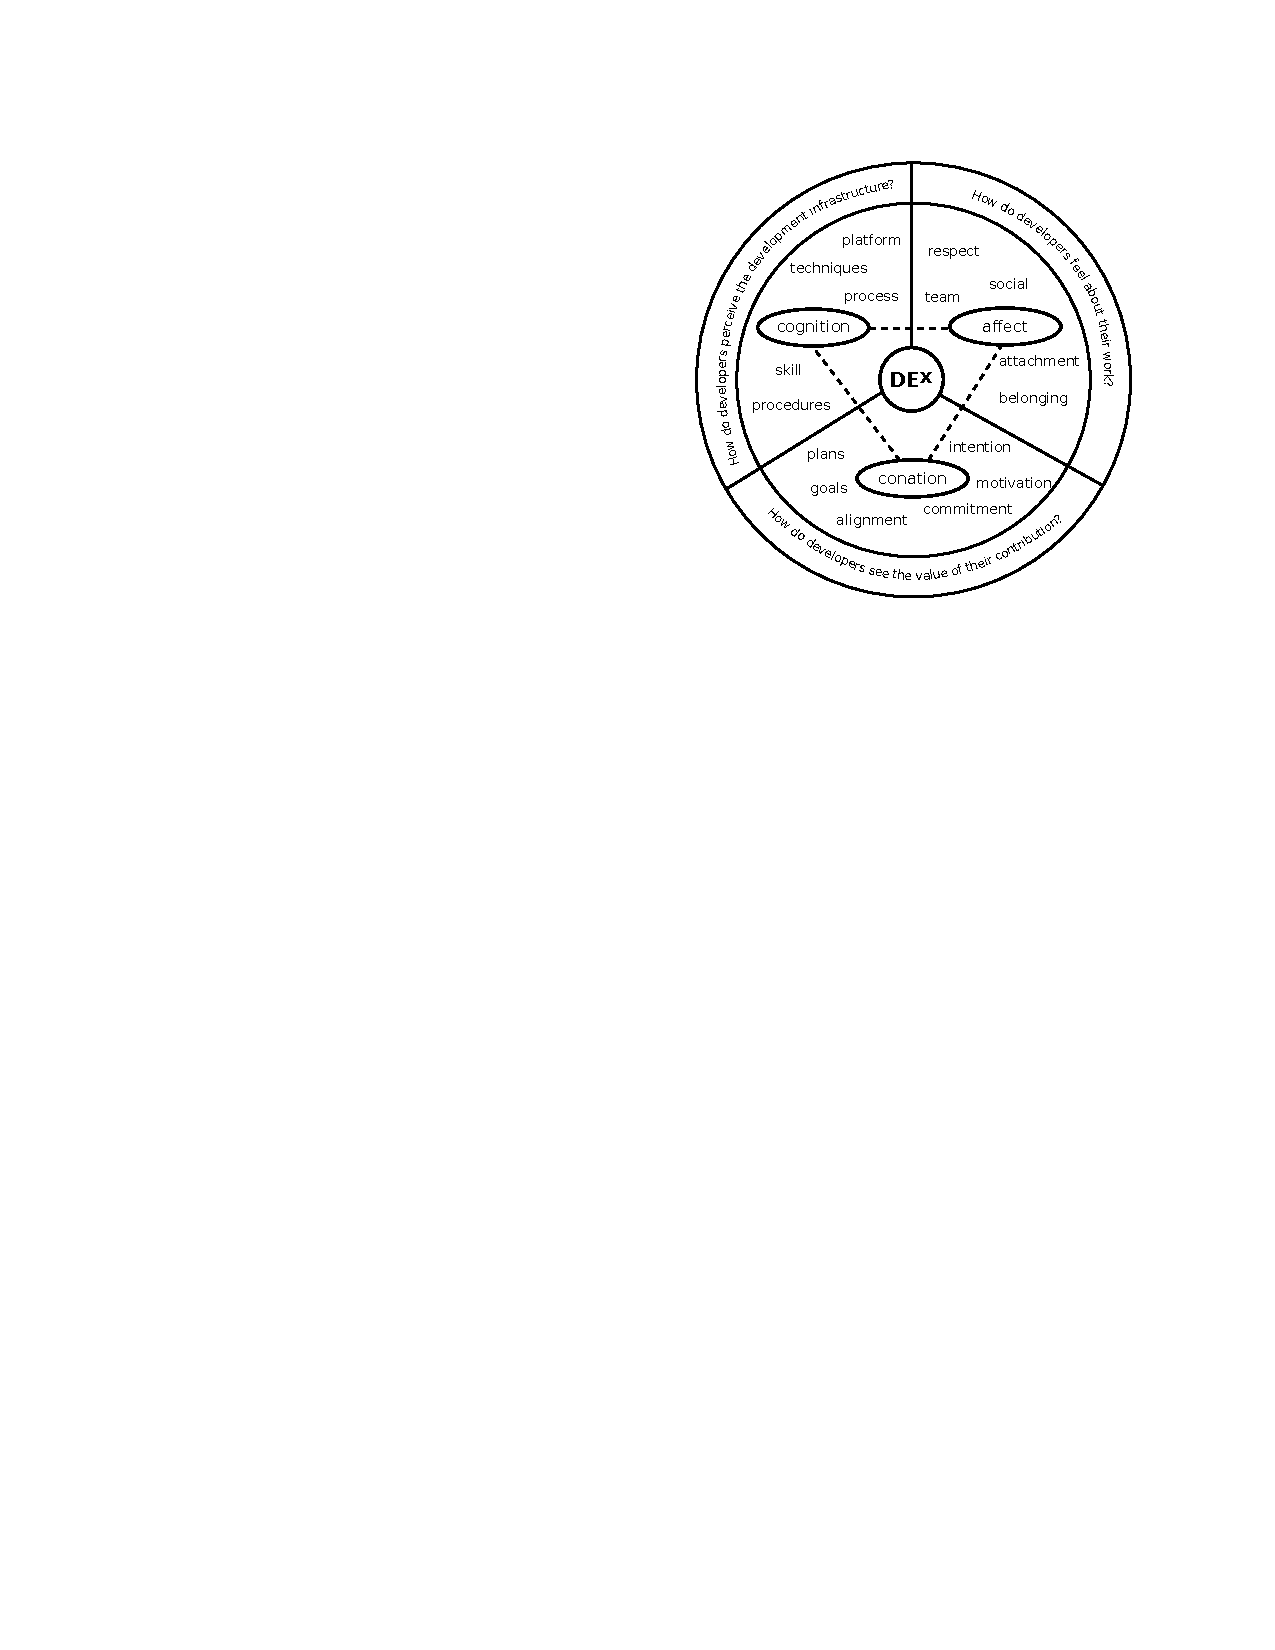
\includegraphics[width=0.6\textwidth]{dx-conceptual.pdf}
  \end{center}
  \label{figure:conceptual-framework}
\end{figure}

\begin{figure}
  \captionsetup{width=0.6\textwidth}
  \caption{The Developer Experience Concept \parencite{fagerholm-doctoral-thesis}}
  \begin{center}
    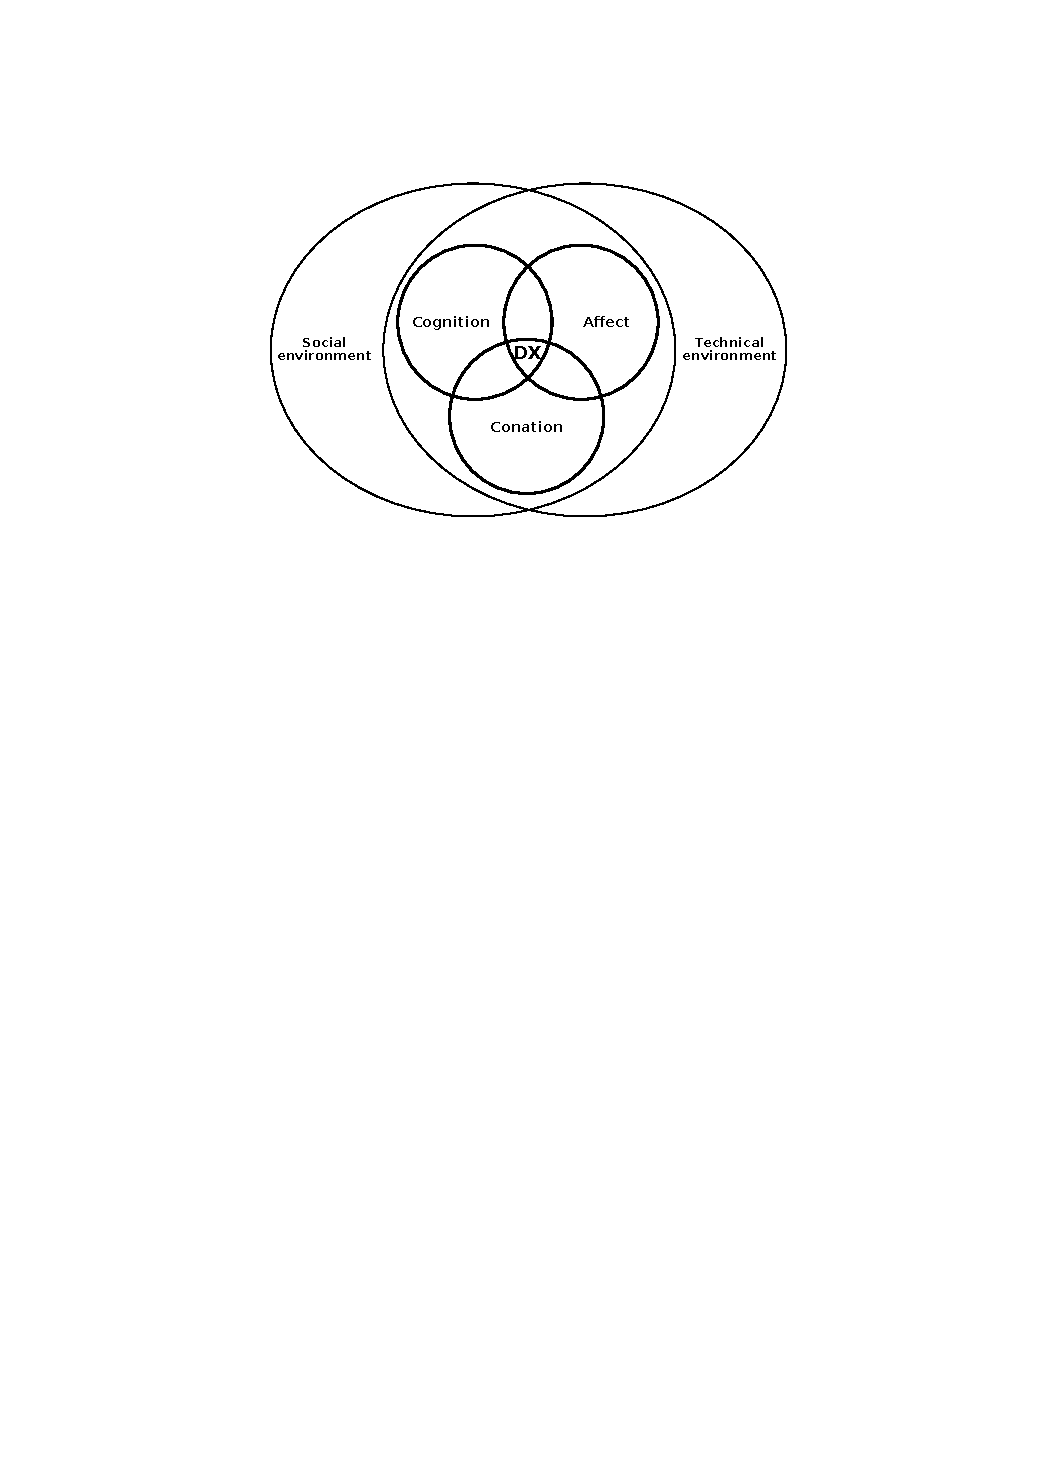
\includegraphics[width=0.6\textwidth]{dx-social-technical.pdf}
  \end{center}
  \label{figure:social-technical}
\end{figure}



Social aspect of software development plays a crucial role on how a developer experiences the development practice, and is receiving as much consideration as the technical environment in figure \ref{figure:social-technical}. It has for long been noted that the social and human factors of software development are not considered as important as they should be \parencite{human-factor}.

The technical environment, including programming languages, infrastructure, processes, techniques, plans, diagrams etc., is also part of the DX. A developer is interacting with these artifacts and that generates an experience. Activities with these artefacts are both experienced as an individual but also as an group.

Time-wise, the DX can be both short term impulsive, or related to one event in software development, but it can also be a long term experience over a period of time, in e.g. a software project.

\textcite{fagerholm-dx-concept-and-definition} takes an approach from psychology, and divides DX into three different sub areas or categories – cognitive (How developers perceive the development infrastructure), affective (How developers feel about their work), and conative (How developers see the value of their contribution). This conceptual framework is presented in figure \ref{figure:conceptual-framework}.

DX can be seen as important from multiple different viewpoints. From a viewpoint of project management a better DX can help to understand, evaluate, and plan projects so that they are inline with the three different dimensions of DX. Another viewpoint is when designing a software development platform or environment, it can be beneficial to understand what impacts and affect the DX, so that the platform or environment can be designed to be aligned with the developers using it \parencite{fagerholm-dx-concept-and-definition}.

% TODO: \textcite{exploring-peopleware-in-cd}

\begin{figure}
  \captionsetup{width=0.6\textwidth}
  \caption{Theoretical Framework of Developer Experience \parencite{fagerholm-doctoral-thesis}}
  \begin{center}
    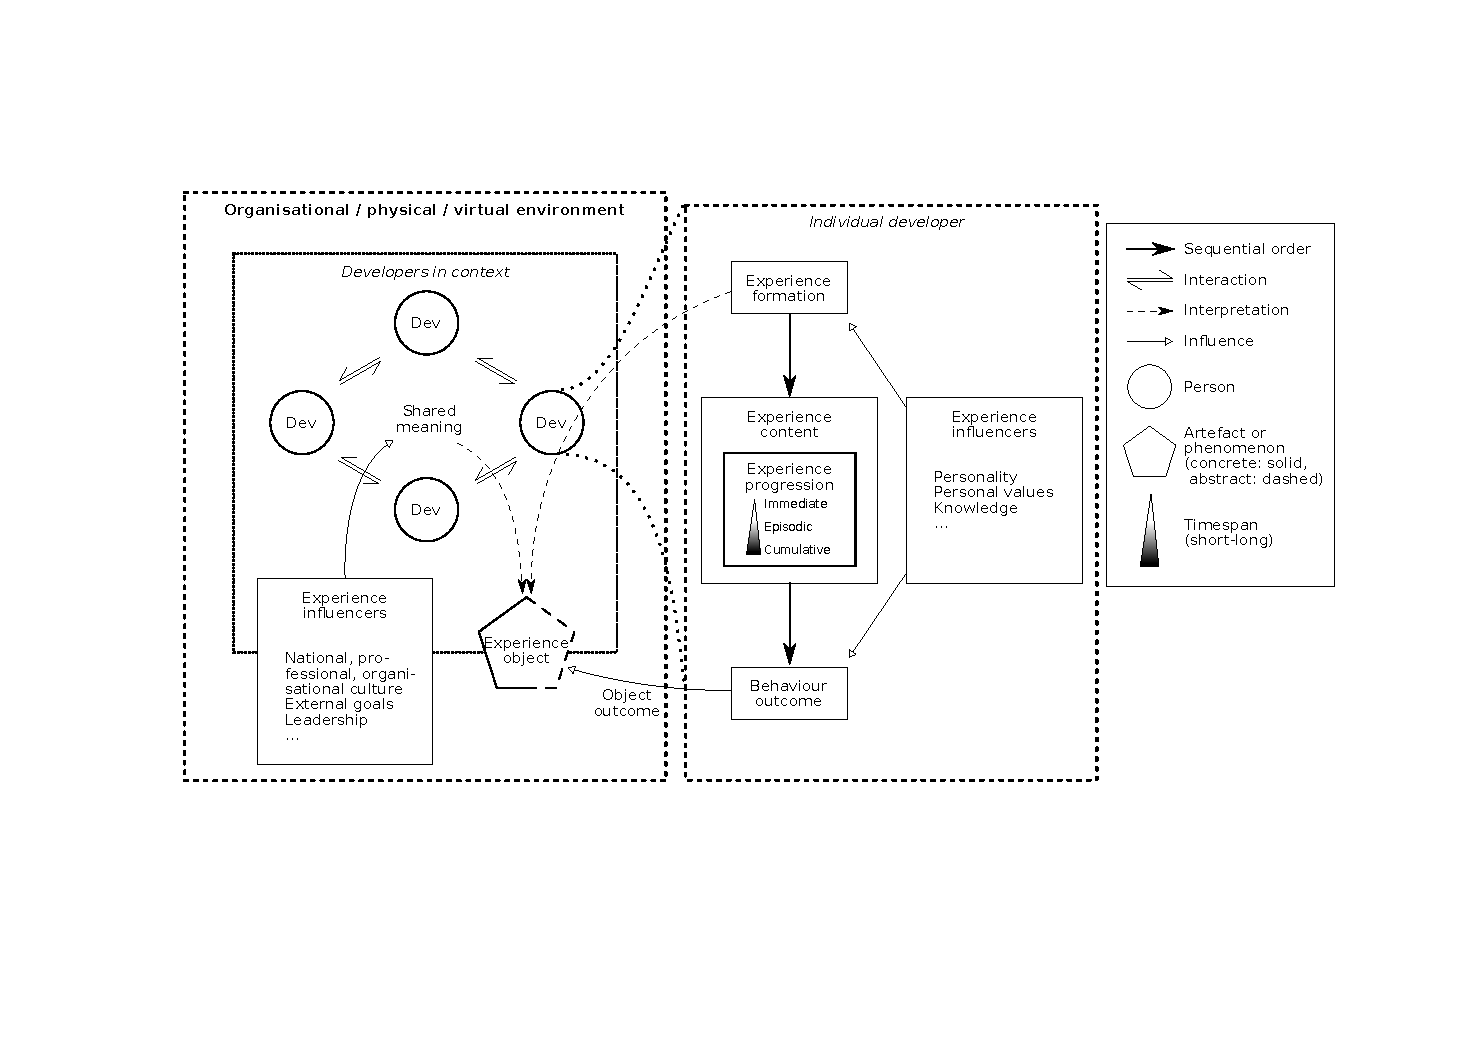
\includegraphics[width=\textwidth]{theoretical-framework.pdf}
  \end{center}
  \label{figure:theoretical-framework}
\end{figure}

The theoretical framework by \textcite{fagerholm-doctoral-thesis} presented in figure \ref{figure:theoretical-framework} is a presentation of the activities of developers in a individual and social environment, and how the experiences arise. The framework is includes aspects as experience \textit{objects, formations, influencers, content, progression},\textit{behaviour outcome} and \textit{object outcome}. These different aspects can be used to study DX from a wide variety of different viewpoints.



\subsubsection{Programmer Experience}

A software developer is a person with a bigger responsibility than a programmer. If a programmer is following instructions, requirements, and guidelines, the developer is also finding out what the instructions, requirements and guidelines should be and probably also helps in defining them. Therefore DX is also considering more of the surrounding context than what Programmer Experience (PX) is considering.

DX and its related terms have been studied and researched relatively little at the moment of writing (\now). \textcite{programmer-experience} performed a literature review of the term \textit{"Programmer Experience"}, that studied 73 articles that matched their defined search criteria. The study concluded that there is still some ambiguity in the term \textit{Programmer Experience} in the context of programming environments, design documents, and programming codes.

Developer Experience (DX) is a bigger construct than PX. DX includes also the motivation of developers, and not only the artefacts like the programming environments \parencite{programmer-experience}. Developer Experience is considering also the social aspect of being a software developer. Developer Experience is what is felt by the developer while trying to achieve a goal i.e. completing a project

Programmer Experience (PX) can be defined as \textit{The result of the intrinsic motivations and perceptions of programmers about the use of development artifacts} \parencite{programmer-experience}. A programmer can be seen as person who gives exact instructions on how a program should behave and function. PX is based on the study mainly related to the programming environment, but also programming codes and Application Programming Interfaces (API).

% http://programming-experience.org/px19/ https://2019.programming-conference.org/

\subsubsection{User Experience} \label{section:ux}

User Experience (UX) emerged from the traditional field of HCI. It was seen that only focusing on the instrumental value of the product or service is not enough. \textcite{ux-research-agenda} studied recent research of UX, and also proposed the future of it to aid in finding a direction for research of it. They found 3 important perspectives of UX. 1) UX is beyond the instrumental by considering the holistic, aesthetic, and hedonic aspects of usage. 2) Emotion and affect are to interest when understanding the subjective view on usage, that often is focused on the positive antecedents and consequences. 3) The experience in itself is a complex and dynamic phenomena that is near to impossible to replicate.

\textcite{understanding-ux} found that the notion of User Experience (UX) has been widely adopted, without having a clear understanding and definition of what UX. Interestingly,this relates exactly to the situation that DX is in now.

\subsubsection{User Starting Experience}

\textcite{api-designers} introduce the concepts of \textit{0 to 200} and \textit{Time to Hello World}. These both concepts are discussing the approachability of APIs. Developers have become more and more in charge of the decision and selection of the tools and 3rd party products that are used when developing software. This might have been more of a responsibility of the organization or the directors or managers before. Now however, it has been seen that the developers are the most knowledgeable persons to make these decisions. \textcite{api-designers} argue that the first encounter with the API determines if it's selected for usage or not, especially if there is a set of different options to choose from. Therefore they also say that the \textit{0 to 200} and \textit{Time to Hello World} are important things to consider when developing APIs with a good DX.

\textit{0 to 200} comes from the Hypertext Transfer Protocol HTTP code 200 indicating a successful OK response. Adopting a new API and successfully calling the API with a 200 OK response can be seen as the minimal effort to get the integration working.

\textit{Time to Hello World} comes from the introduction and adoption a new programming language, where often the first task is to print or log the string "Hello World" to the console or terminal. Adopting the basic structures and building block of the programming language prove how easy it is to get going with it, and therefore can be a measurement of the approachability of the language.

However, this shouldn't be limited or restricted to only APIs, programming languages, or frameworks. The concept of User Starting Experience could be used in the measurement of introducing or adopting anything new related to software development e.g. a new development technique or process.

\subsection{Selection of tools}

Perceived choice is a perception of that the choice has already been made \parencite{flow-intrinsic-dx}. Selecting tools in software development projects is in a crucial role, as it can significantly improve the Developer Experience in software projects.

\textcite{flow-intrinsic-dx} studied Integrated Development Environment (IDE), and how they are connected with state of flow, intrinsic motivation, and user experience. Their findings reveal that if the developers have a high perception of choice, the also are overall more satisfied with the tools. They also concluded that if the selected tools are selected without their input, (they perceive it chosen already), the developers will have a worse developer experience with it, as e.g. their frustration with the tool will be more common.

There has been a study on the Developer Experience of IDEs \parencite{software-developers-as-users}. However, the study concentrated on the UX of the selected IDE that was studied.

When selecting an IDE it is also important to consider what the other developers in the team or organization is using or what other would prefer to use.

\textcite{design-framework-enchancing}

There can be situations when two different developers use a different IDE, and therefore also the experience can be completely different between them. At the most extreme the 2 IDEs are not compatible with each other as their files related to the project are different. An example of this is Eclipse and IntelliJ IDEA as Java IDEs.

In a study of IDEs \parencite{software-developers-as-users}, the survey in the study produced answers that were most pragmatic, but not hedonic. This could show that most of the developers are practical, and not feeling based. This has also been proven \parencite{personality-software}. This might also be a reason why Developer Experience has not gotten that much attention yet, as big part of people in software engineering are \textit{"Introverts"}. Software engineers are also more logical thinkers than feeling based. As Developer Experience is focusing on the feelings and subjective opinions about things, it might be a difficult topic to research.

\subsection{Organization and project onboarding}

\textcite{entering-an-ecosystem} have studied the process of entering an ecosystem from the perspective of developers. They have especially focused on the onboarding process of Hybrid Open Source Software projects that have special characteristics as software projects.

Open Source Software (OSS) is software developed, where the source code of the software is accessible to the public. OSS is often developed by a community where anyone participating is allowed to report problems, suggest changes, and also modify the code and develop the software. However, the fact that anyone interested can participate in the community results in that the communities often create their own complex organization and hierarchy.

A hybrid OSS can consist of individual developers, but also sponsored and supported developers that are pursuing the interests of some other organization. One example of this is JavaScript framework React, that was initially developed at Facebook, but later open sourced. Hybrid OSS creates another layer of complexity of the organization.

\textcite{entering-an-ecosystem} argue that onboarding and welcoming new developers to hybrid OSS might be more difficult than normal OSS projects. All in all, onboarding of any kind of software project is part of the whole DX of the onboarding developer.

\subsection{Motivation}

Intrinsic Motivation (IM) is the motivation that is enabled by someone enjoying their own work, i.e. the motivation is originating from the work itself. Extrinsic Motivation (EM) is motivation that stems from the outcomes of the work performed \parencite{flow-intrinsic-dx} (Self-determination theory. Handbook of theories of social psychology).

\subsection{Performance Alignment Work}

\textcite{how-developers-experience-team-performance} and \textcite{paw} have created a framework called Performance Alignment Work (PAW), that explains the phenomena of experiencing performance in software development context. Software development performance is a complex construct where performance measurement is not a straightforward practice.

The PAW framework acknowledges that performance can not be measured trough some objective measures, as there are too many different viewpoints to measure software project performance from. It also acknowledges that performance exists on multiple different levels e.g. individual, team, organization, or customer level. Their study concluded that high-performing teams are considered high-performing because the are able to alter the ways the performance of the team is measured.

The performance of a software development project is highly linked with the DX of the individual and the whole team, and \textcite{how-developers-experience-team-performance} suggest that by aligning affective and conative aspects with individual developers and within the whole software development team, there could be opportunities to reach improved performance.

\subsection{Happiness of developers}

Happiness of developers has been reported have high impact on the practice of software development and have consequences. A series of studies, namely \textcite{unhappy-developers}, \textcite{on-the-unhappiness}, \textcite{consequences-of-unhappiness}, and \textcite{what-happens-when-unhappy} studies the happiness and unhappiness of developers. They concluded that the (un)happiness of the developer has consequences on the themselves, the process, and the end product. The concept of DX \parencite{fagerholm-dx-concept-and-definition} includes the affective dimension that is directly related to the happiness of developers.

\subsection{Flow state}

The flow state is a state where the task at hand has gotten full attention \parencite{flow-intrinsic-dx}. Flow state is something that many developers want to achieve. For some developers it is really difficult to focus if there are external things that disturb them like sound or something similar. Also, people coming and asking questions might disturb or interrupt the flow state. Therefore many developers are now also trying out remote work where they are not co-located. Achieving flow state requires a clear set of goals, continuous feedback, and a good balance between skills and challenge.

\subsection{Application Programming Interfaces}

Application Programming Interfaces (APIs) are interface that developers use to communicate and transfer information with external service, but also to build products and services with. As developers are in the role of using APIs, the APIs UX, and also DX, has been researched \parencite{api-designers}. Developers are the main users of APIs, the API's DX has been considered as a very important aspect of the API. A good DX aids in getting users for an API.

APIs, and especially Web APIs have enabled to create businesses around APIs \parencite{api-ecosystem}, \parencite{web-api-economy}, \parencite{moilanen2018api}. This type of business is called an API economy, and has quickly become a viable way of generating revenue for businesses.

\clearpage
\section{Research methods}

During the study, the research problem and the research questions evolved as the understanding and comprehension of the problem improved. Because of this the planned research methods and the goals with these also evolved and were reshaped when new information was acquired. From the introduction and motivation in sections \ref{introduction} and \ref{motivation}, it was determined that DX is a novel and abstract construct. The concepts and definitions of it are multiple, and vary both in research and in industry. This means that the author's understanding of the topic improved and evolved during the study.

\textcite{easterbrook2008selecting} define a set of guidelines for empirical research in software engineering. They argue that selecting a clear research question, an explicit philosophical stance, and an appropriate research method are key when researching in the context of Software Engineering (SE). They also note that many research projects in SE fail in defining the stance of the research, which then further complicates all aspects of the research including its interpretation, validity, replicability etc.

During writing of the thesis, the author was working at the case company, allowing to perform ethnographic techniques in understanding and studying the phenomena. Working at the case company also allowed to have discussion with colleagues.

\subsection{Research approach}

This thesis takes an exploratory approach to study the research problem and to answer the research questions. A research with an exploratory approach considers questions that address the existence of a phenomena, try to describe something \parencite{easterbrook2008selecting}. The definition of DX given by \textcite{fagerholm-dx-concept-and-definition} (figure ) and \textcite{fagerholm-doctoral-thesis}, and they function as the basis of the study, but they are only giving the abstract concept to build upon. This concept and framework has not yet been widely taken into practice in empirical research. From \textcite{fagerholm-doctoral-thesis} the theoretical framework was used for guiding the research. 

Also, from initial discussion in the case company there was almost as many definitions of DX as there was discussions. This shows that depending on the role of the practitioner and the context they are working in affects in the definition of DX.

In \textcite{developing-grounded-theory} Juliet Corbin reflects on the grounded theory research methodology and how she approached a research she conducted in combination while writing a book \parencite{basics-of-qualitative-research} about grounded theory.

\begin{quotation}
  \textit{"I was just going to sit down with that first piece of data in front of me and let it flow, let the research take me where it wanted"} - Juliet Corbin \parencite[p.~43]{developing-grounded-theory}
\end{quotation}

Taking an approach that enabled an open mindset allowed to question suitable research questions, and this approach was the most suitable in this thesis, both from the viewpoint of the research topic and researchers own skills, competency, and way of thought.

% TODO: Read "Grounded theory in software engineering research: a critical review and guidelines"

\subsection{Research philosophy} \label{section:research-philosophy}

According to \textcite{easterbrook2008selecting}, making explicit decisions on the research methods is key, and by doing that the research becomes more beneficial for practitioners and other researchers. Therefore they also argue that explicitly defining every step of the research should be done.

This thesis will take a \textbf{constructivism} view of the truth, combined with pragmatic approach. A constructivist approach sees the problem as that the human context is always present, and that it is an important part of the research and the study. The \textbf{pragmatic} approach is also required because of the case company in this study. The context of a company is important to include, as something that works with one company, might not work with another company. The pragmatic approach can be seen as an approach from engineering, where the interest is focused on what works at a specific time in a specific context.

An \textbf{positivism} is not a suitable approach in this context. A positivistic approach tries to build up knowledge on verifiable observations that is then incrementally built upon. Positivists prefer to create specific theories from where testable hypotheses are extracted. These hypotheses are then tested in an controlled and isolated environment \parencite{easterbrook2008selecting}.

\subsection{Unit of analysis}

\textcite{easterbrook2008selecting} point out that it is important to pick the unit of analysis of the study. The unit in this case could be a company or organization, a project, a team, or an individual software developer. As DX is the experience of an individual developer, it is selected as the primary focus in this study.

Another viewpoint to this is also the case company, that has its own culture and set of practices. This study will also see the company as a unit of analysis. The company culture and practices are something that is shared between every developer and other employees.

\subsection{Research method selection}

To be able to investigate and define the definition of DX at the case company, the study has to focus on the foundations. During early stages of the thesis, it was noted that a comprehensive literature review and study was required. A good literature review gives a good foundation on which to build the research upon, and ensures that the studied field is understood correctly.

\subsubsection{Multivocal Literature Review}

Each research and study should have a background check and literature review where previous material and research is assessed, and from where the current research can be continued and built upon. A MLR is a form of systematic literature review, that produces both qualitative and quantitative data. In this study a MLR was seen as a good fit, as it allows to get a broad view of the current state of the research in the topic. It also allows to answer exploratory questions where the existence of a subject or topic is abstract or vague. A more comprehensive discussion of the MLR is discussed in section \ref{mlr}.

% TODO: is this subsection of MLR required here or can it be discussed completely in the section of MLR?

\subsubsection{Brainstorming}

Brainstorming (BS) is a widely used technique, where the idea is to foster unique and novel ideas. Usually BS sessions are conducted when there is a need for innovation and new ideas. One typical use case of BS would be in a context of developing a product. With help of involving the development team in a BS session, new ideas and possible development directions can be found. The foundation of BS lies in that there are no right and wrong ideas, and that every idea is welcome.

In the context of this thesis, the technique of BS works as an exploratory way of initiating the study. Because of the novelty of the research topic DX, BS is an appropriate way of establishing the initial understanding of DX in the context of the study and the case company. Because the researcher has created their own understanding of what DX is, it would interfere with the study results if the researcher would participate into the sessions. It would also be problematic if the researcher would introduce the topic before the session, because the would either change or deepen the personal image of DX that the participants at that moment have. This is in line with the exploratory research philosophy described by \textcite{ethnographically-informed}. If the initial session would have been for example a workshop facilitated by the researcher, the researcher might have affected the session, and it would not have yielded in the same results as with a BS session.

Brainstorming types can be identified into \textit{Traditional Brainstorming (TBS)}, \textit{Nominal Brainstorming (NBS)}, \textit{Electronic brainstorming (EBS)} \parencite{brainstorming-techniques}. \textit{TBS} are verbal brainstorming sessions where the idea is to brainstorm verbally together in a group face-to-face. \textit{NBS} can be seen as individual BS sessions, where each individual does the brainstorming without working together. \textit{EBS} is a way to conduct BS with help of computers, from where each individual can concurrently input their ideas. Meanwhile the participants can see ideas from others. However there is a level of anonymity that defeats some of the problems with TBS and NBS.  All in all, the different types of BS has been studied and their efficiency is dependent on many factors \parencite{productivity-loss-in-brainstorming-groups}, \parencite{electronic-brainstorming}, \parencite{chainstorm}.

There are some problems with brainstorming sessions \parencite{electronic-brainstorming} \parencite{chainstorm}. \textit{Evaluation apprehension} means that group members might get the feeling of being judged, and therefore they might feel reticent with bringing out their ideas. \textit{Production blocking} might also be a problem, as working in groups will require everyone to talk on their own turns, which might lead to ideas becoming irrelevant, ideas might be forgot, the ideas might be rehearsed that blocks the generation of new ideas. \textit{Free riding} can also happen when some BS group members rely on other members to perform the BS actions. According to \textcite{six-issues-of-brainstorming}, the proponents of brainstorming is the practitioners, and the opponents are often researchers.

In this study the initial brainstorming session was selected to be a combination of TBS and NBS. NBS allows everyone to work individually. The case company has also established itself as working very agile, and therefore mentioned problems with BS do not require any extra actions to mitigate them. The BS session used Think-Pair-Share method \parencite{think-pair-share}, where each participant of the session first thinks about the problem and possible ideas by themselves, then after that each individual is paired together where they share their own initial ideas, discard duplicate ideas, and further develop new ideas after the discussion. After pairing, each pair presents their ideas and findings to the whole group.

% \subsubsection{Interviews}

% Interviews can be conducted with the concept and framework of developer experience, even without having the participants being aware of the definition of Developer Experience. By using the conation, affection, and cognition, it is possible to initiate discussions of the different elements of DX.

% Write a lot more about interviews
% Topics to address:
% - What is the goal of the interviews? 
% - What data is going to be collected from the interviews
% - Semi-structured interviews or some other research approach for the interviews?

\subsection{Timeline}

Mixed-methods approaches are more complex research strategies where multiple different approaches of an empirical study is combined \parencite{easterbrook2008selecting}. In mixed-methods approaches the limitations of the different methods are acknowledged, and the limitations of them are mitigated.

\textit{Sequential exploratory strategy} is one specific mixed-methods research approach. In this approach first qualitative data is collected and analyzed, after which the focus shifts towards quantitative data. Purpose of this approach is to first explore the topic with help of qualitative research, and then possibly test some emerging theory with help of quantitative research. Another reason might be to help in interpreting the qualitative data.

\textit{Concurrent triangulation strategy} is another specific approach of mixed-methods \parencite{easterbrook2008selecting}, where different research methods are used concurrently. The concurrent research enables to use results from one method to another, and vice versa. This enables to cross-validate research findings.

In this thesis both \textit{sequential exploratory strategy} and \textit{concurrent triangulation strategy} was used as research approaches. The sequential exploratory strategy was implemented by first conducting the initial multivocal and traditional literature reviews, and then only after that the ideation and planning of the workshops started. However at this point the MLR was not finalized, and still had some open questions, and ongoing interpretations and analysis.

The technique of concurrent triangulation strategy was utilized by conducting the MLR and the brainstorming concurrently. While the first iteration of the MLR was being performed, the initial workshop at the case software consultancy company was held. The idea behind a concurrent research was to get as comprehensive definition of the research problem as possible from as many different viewpoints and contexts as possible.

The initiation of the thesis started during the summer of 2019. The topic of the thesis was selected, and the initial and the preliminary research question and problem were defined. At that moment, the concept of DX was too vague to the author. After some discussions and studies on the topic, it was decided that the MLR should be taken as the first step of the study. When the MLR had been initiated the first results from it emerged, at the meantime the context of the empirical study started also to get defined.

\subsection{Analysis of data}

\textcite{analyzing-qualitative-data} give a set of guidelines and practices on analysing qualitative data. They state that using qualitative data in research requires discipline, creativity, but also a systematic approach. The divide the analysis of qualitative data into 5 different step: get to know your data, focus the analysis, categorize information, identify patterns and connections within and between categories, and finally interpretation. Categorization of the data is explained more in the specific sections where categorization, theming, or coding of data is performed.

\clearpage
\section{Multivocal literature review} \label{mlr}

Traditionally, in Systematic Literature Reviews (SLR) the reviewed literature consists only of literature that is formally published, and of which the motivation of publishing is the publication in itself, e.g. scientific publications in journals and conferences. Material that is produced with commercial interests and informally published material and publications are not considered in SLR \parencite{guidelines-for-MLR}.

Multivocal Literature Reviews (MLR), are a way to include grey literature into SLRs \parencite{the-need-for-MLR}. Grey literature can be defined in different ways, and research fields define grey literature in ways that are meaningful to that specific field.

\begin{quotation}
  \textit{"Grey literature stands for manifold document types produced on all levels of government, academics, business and industry in print and electronic formats that are protected by intellectual property rights, of sufficient quality to be collected and preserved by library holdings or institutional repositories, but not controlled by commercial publishers i.e., where publishing is not the primary activity of the producing body."} \parencite{towards-a-prague-definition-of-grey-literature}
\end{quotation}

The Prague Definition of grey literature is strict and therefore not allowing e.g. blog posts to be used on MLRs. However, a specific guideline for including grey literature in literature reviews has been created \parencite{guidelines-for-MLR}. This guideline is based on the guidelines on how to perform SLR in SE \parencite{guidelines-for-SLR-in-SE}.

\subsection{The motivation behind a Multivocal Literature Review}

DX is an abstract concept and framework. As pointed by \textcite{fagerholm-doctoral-thesis}, the framework they present can be used to guide inquiries into DX. There was a need to create an understanding of the definition of DX from the point of view in this thesis. Traditional literature reviews can help in these cases, and they create a common understanding and basis of the topic that is going to be discussed. However, traditional literature reviews are prone to be biased. To avoid bias of the author, and because DX is a subjective concept of the developer, the definition of DX could have been reviewed with a help of a SLR. SLRs are a way of producing evidence based results, and they are effective in complex and opinion based fields where a common agreement of a concept or topic might be difficult to find.

In software engineering practitioners constantly produce valuable literature in e.g. technical reports or blog posts, but this material is not considered in SLRs. This has been identified as a problem, and there's been a call for MLRs in SE \parencite{the-need-for-MLR}. An SLR would include only the scientific papers, and therefore it might not be sufficient to only focus on that. In a MLR the GL should provide a current perspective and fill in the gaps of scientific and formal literature \parencite{guidelines-for-MLR}. SE practitioners are producing a lot of literature, that would not be considered in normal literature reviews or SLR. This GL can provide insights about the field of SE, and especially about DX.

% TODO: Read \parencite{guidelines-for-MLR} again after reading \parencite{guidelines-for-SLR-in-SE}.

\subsection{The review protocol of the Multivocal Literature Review}

DX is a novel concept, and therefore there has been little formal research on the topic. Based on the different levels of literature, white, grey, and black \parencite{guidelines-for-MLR}, DX could be seen even to be in the category of black literature. DX can still be seen to be on the level of ideas, concepts, and thoughts.

\newcommand{\mlrdxlink}{https://bit.ly/31QzQ7z}

All data of the MLR can be found the following link: \href{\mlrdxlink}{https://bit.ly/31QzQ7z}. The data collection is done with Google Sheets and is based on the example shown in \parencite{guidelines-for-MLR}.

\subsubsection{Research questions}

The foundation for the MLR is the first research question \hyperref[RQ1]{RQ1} (\rqone). The goal is to create a understanding of the current situation of the definition of \textit{Developer Experience} with help of both white literature and grey literature.

\subsubsection{Search process}

The search process was divided into a database search and a snowballing procedure performed on the first initial set of the results. The following sections motivate the decisions made before and during the search process, and explain the details on how the search was conducted.

\subsubsubsection{Database search}

The first iteration of the search was performed as a manual search by the author from various libraries to gather the scientific literature. For grey literature, the Google search engine (https://www.google.com) was be used. To limit the amount of results in the search of grey literature, only the first 2 pages of searches from google.com will be included. In a study conducted by \textcite{google-search}, only 91 percent of participants in a study went to the second page of google results page. Therefore it's appropriate to include only the most relevant (the first pages of the results) results from the google search. The selected databases and libraries of sources of scientific literature is listed in table \ref{table:included-databases}.

\begin{table}
  \centering
  \begin{tabular}{ l l }
    \hline
    IEEExplore    & https://ieeexplore.ieee.org/Xplore/home.jsp          \\
    ACM           & https://dl.acm.org/                                  \\
    ScienceDirect & https://www.sciencedirect.com/                       \\
    Scopus        & https://www.scopus.com/search/form.uri?display=basic \\
    \hline
  \end{tabular}
  \caption{Databases used for the MLR}
  \label{table:included-databases}
\end{table}

\begin{table}
  \centering
  \begin{tabular}{ l l }
    \hline
    Google Scholar & (https://scholar.google.com)          \\
    Citeseer       & (https://citeseerx.ist.psu.edu/index) \\
    SpringerLink   & (https://link.springer.com/)          \\
    \hline
  \end{tabular}
  \caption{Databases excluded from the MLR}
  \label{table:excluded-databases}
\end{table}

Other possible libraries and databases that could have been used are listed in table \ref{table:excluded-databases}. However, the sources listed in this table does not provide advanced search. Advanced search by author keyword was a search criteria and because of that these libraries and databases were excluded from the initial search of sources.

\textcite{guidelines-for-snowballing} state that with manual searches of sources, the results will vary and are hard to replicate because of the lack of a system. This is key when performing systematic reviews so other researchers can replicate the study. \textcite{guidelines-for-snowballing} also mention that performing database searches might result in a big set of irrelevant results, from where it can be difficult to find the relevant result from. The process of manually filtering out results is also error prone.

Search string for both scientific and grey literature was \textbf{"developer experience"}. The aim of the MLR review was to get an overview of the definition of DX, only that specific search string was used. That assured that all relevant publications were included. Including more words in the search string or creating a more complex search string would have required a better understanding of DX. Also, including other search strings would have biased the search result. To further narrow down the search, the search was modified to include only results where author keyword was "developer experience". This narrowed down the search significantly, and removed irrelevant results. \textcite{guidelines-for-snowballing} mention that creating complex queries and search strings might be difficult because of the lacking standardized terminology of the research topic. This was exactly the case with this study, as the topic of DX is relatively novel and some research might be studying DX without explicitly stating or even being aware of that themselves.

Using the author keyword gave results where the author is intentionally discussing the topic of DX. In the case of DX, with searching only with the author keyword, the inclusion/exclusion rate is significantly better than with a full-text search. However, this approach removed the possibility to discover definitions of DX where the author is not aware of this concept or phenomenon.

\textcite{understanding-ux} performed a search on the definition of UX. Their search strings used a combination of keywords. However, trying to replicate these for the search of the definition of DX did not yield any satisfactory results, and either the number of search results was too big or too small.

\subsubsubsection{Snowballing}

The result of the database search gave good results that however were too narrow. With the guidance of the thesis supervisor who has done extensive research on DX, the decision of using snowballing to collect more sources was done. Snowballing allows to find sources that would otherwise go undiscovered. For example obscure journals, conferences, or magazines can be difficult to find with only using database searchers \parencite{guidelines-for-snowballing}.

In this thesis one iteration of snowballing was performed on the scientific articles. The first set of scientific literature included 21 articles. Snowballing was performed on these 21 articles, and the first round of backward and forward snowballing resulted in 5 articles from backward and 14 articles from forward snowballing. Snowballing on

Snowballing was not used on grey literature. However, 2 different searches with the same keyword was performed in Google Search. The first round of grey literature about the topic was gathered at September 2019, and the second round in November 2019. Having two different occasions of gathering grey literature sources did take into action timely changes in search results of Google.

\subsubsection{Inclusion criteria}

The included material had to be written in English. Articles that showed up in the searches, and that had the words \textbf{developer experience} in consecutive order, were included in the review. This inclusion criteria of having the term "developer experience" was applied both the database search and the snowballing technique.

The selected sources had to discuss about DX explicitly mostly by using the term as it is. Without this criteria it would have been a complex job to draw a line between inclusion and exclusion, as basically every study concerning software engineering to some degree is more or less related to topic of DX.

\subsubsection{Exclusion criteria}

Papers that discussed about developer's experience in terms of the experience level were excluded from the review. These included papers where developers were compared on the experience level e.g. \textit{senior} or \textit{junior developer}. Also, where experience is defined as number of years working in software development or the number of commits in a software commit were excluded.

% \subsubsection{Primary study selection process}

\subsubsection{Quality assessment}

\textcite{guidelines-for-MLR} give guidelines on how to assess the quality of the sources. This can be done with help of quality points based on some set of questions or points of measure. This is useful when the aim is to achieve a certain level on the sources. It also helps to filter out a big number of possible sources. Because of the novel topic the quality assessments were not considered in this study. The amount of sources were low and because of the exploratory nature of the study, every possible and available source were considered.

\subsubsection{Data collection}

All sources of the review were collected into one form with the selected data points. The process of collection was a continuous refinement of the search method, inclusion and exclusion criteria, and data extraction points. During the collection the comprehension and understanding of the base concept of DX was continuously refined. The author's understanding about the topic improved, and therefore there was also need to continuously update and refine the data collection form.

First version of the data collection form was simple and included only some basic characteristics and data points of the sources. With help of ongoing collection, refinement of the search process, and adjustments to the research questions the data points emerged to their final form. A more comprehensive explanation of the collected data points is given in section \ref{section:result-of-mlr}.

% TODO: reassess if the table below should be included or not

% \begin{table}
%   \begin{center}
%     \begin{tabular}{ | p{0.4\textwidth} | p{0.5\textwidth} | }
%       \hline
%       \textbf{Data point}                                     & \textbf{Description}                                                                                                                                                                                          \\ \hline
%       Title                                                   & Title of the source                                                                                                                                                                                           \\ \hline
%       Link to the source                                      & http-link to the source                                                                                                                                                                                       \\ \hline
%       Library                                                 & The library from where source was found                                                                                                                                                                       \\ \hline
%       Year of publication                                     & Year of publication                                                                                                                                                                                           \\ \hline
%       Type of article                                         & Type of article                                                                                                                                                                                               \\ \hline
%       Scientific / grey literature                            & Classification if scientific or grey. Coded as 0 or 1                                                                                                                                                         \\ \hline
%       Author affiliation                                      & Academic, industry, or collaboration                                                                                                                                                                          \\ \hline
%       Research problem / questions / topic                    & The research problem or questions under study                                                                                                                                                                 \\ \hline
%       Research method                                         & The research methods used in the study or article                                                                                                                                                             \\ \hline
%       Object / entity of DX under study                       & Description of the experience object that is being studied                                                                                                                                                    \\ \hline
%       Factors that improve or worsen the DX                   & Factors that cause the DX of the object to be better or worse                                                                                                                                                 \\ \hline
%       Conclusions / results                                   & Summary of the conclusions of the source                                                                                                                                                                      \\ \hline
%       Definition of DX                                        & Short summary of what definition of DX is used                                                                                                                                                                \\ \hline
%       Explicit/implicit definition of DX                      & Some papers explicitly give a definition of DX in the text by either referring other papers or giving their own definition, when other papers use DX without definition (assumes the reader knows what DX is) \\ \hline
%       Reason of interest towards DX                           & Why the source is discussing and studying DX                                                                                                                                                                  \\ \hline
%       Context of DX                                           & From which context is DX looked at in the research                                                                                                                                                            \\ 
%                                                               & Definition                                                                                                                                                                                                    \\ 
%                                                               & Development Environment                                                                                                                                                                                       \\ 
%                                                               & API                                                                                                                                                                                                           \\ 
%                                                               & Product or Service                                                                                                                                                                                            \\ 
%                                                               & User Experience                                                                                                                                                                                               \\ 
%                                                               & Team, Collaboration, and Community                                                                                                                                                                            \\ 
%                                                               & Knowledge Sharing                                                                                                                                                                                             \\ 
%                                                               & Language / library / framework i.e. code in general                                                                                                                                                           \\ 
%                                                               & Mood \& Feelings                                                                                                                                                                                              \\ \hline
%       Mentions "Developer Experience: concept and definition" & If the research mentions Fagerholm and Münch's 2012 article                                                                                                                                                   \\ \hline
%       Other notes                                             & Other noteworthy information                                                                                                                                                                                  \\ \hline
%     \end{tabular}
%     \captionsetup{width=0.6\textwidth}
%     \caption{The data collection points of the MLR}
%     \label{table:data-collection-points}
%   \end{center}
% \end{table}


\subsubsection{Data analysis}

Data collection was rather successful and multiple different data points was extracted. These data points were both qualitative and quantitative in nature. During the data collection, the view of the data collection was focused on a horizontal perspective i.e. on source at a time. During analysis the view was flipped to a vertical view i.e. looking at one data point at a time.

The quantitative data analysis was performed with simple aggregations and visualized with help of charts. No specific methods or techniques of quantitative data were used. Iterating on the categories by removing, adding, and combining them, new categories and patterns emerged.

Qualitative data analysis was performed one data point at at a time. Each data point was copied to an excel table where electronic affinity diagramming was performed. Affinity diagramming or the KJ method \parencite{scupin1997kj} is a technique that allows to make sense of qualitative data. The KJ methods allows to understand and interpret data that would otherwise be difficult to make something out of.

The idea is to shuffle statements that are written cards or notes. Next step is to group things that relate to each other together so that "teams" of cards are formed. Then each of these teams are titled, and finally the relations between teams are explained and reported. This method allows to create new interpretations and reveal hidden meaning behind the collected data. This method was suitable for this MLR, as the majority of the data collected was qualitative e.g. statements and loose interpretations from the articles.

\clearpage
\section{Current state analysis}

\subsection{Case company}

Reaktor is a Finnish company that provides consultancy and agency services. The company was founded in 2000 and has since then been a leading IT-consultancy company in the Finnish market. In addition to offices in Finland, Reaktor has offices in New York, Amsterdam, Tokyo, and Dubai \parencite{reaktor-home}. Reaktor has won the Great Place to Work award multiple times in Finland \parencite{reaktor-gptw} and the company is actively improving the wellbeing of everyone at the company \parencite{talouselama-reaktor}.

A significant part of Reaktor's employee's are technical experts, engineers, and developers. These roles include titles as Senior Software Engineer, Full Stack Engineer, Experience mobile developer (iOS/Android), and DevOps engineer \parencite{reaktor-careers}. This makes studying DX at Reaktor an interesting subject of research. Different roles and specialities have their own viewpoints of DX.

\subsection{Developer Experience at Reaktor}

Developer Experience has not been previously explicitly studied at Reaktor. However, during the initial phases of the thesis, the topic of DX in this thesis caused some interesting informal discussions about some problems and occurrences of DX. These discussions varied in length and depth, but allowed to create a good basis for the empirical study at the company.

Discussion channels used at Reaktor are very active, and information sharing is a constant activity. \textcite{thesis-nelli-vilkko} took a deep dive into the ways of of working at Reaktor, and specifically into how agile methods form the experience of work engagement. They also mention that information sharing and knowledge management is something that gets a lot of care at Reaktor.

\begin{figure}[ht]
  \captionsetup{width=1\textwidth}
  \caption{Daily active Slack members at Reaktor}
  \begin{center}
    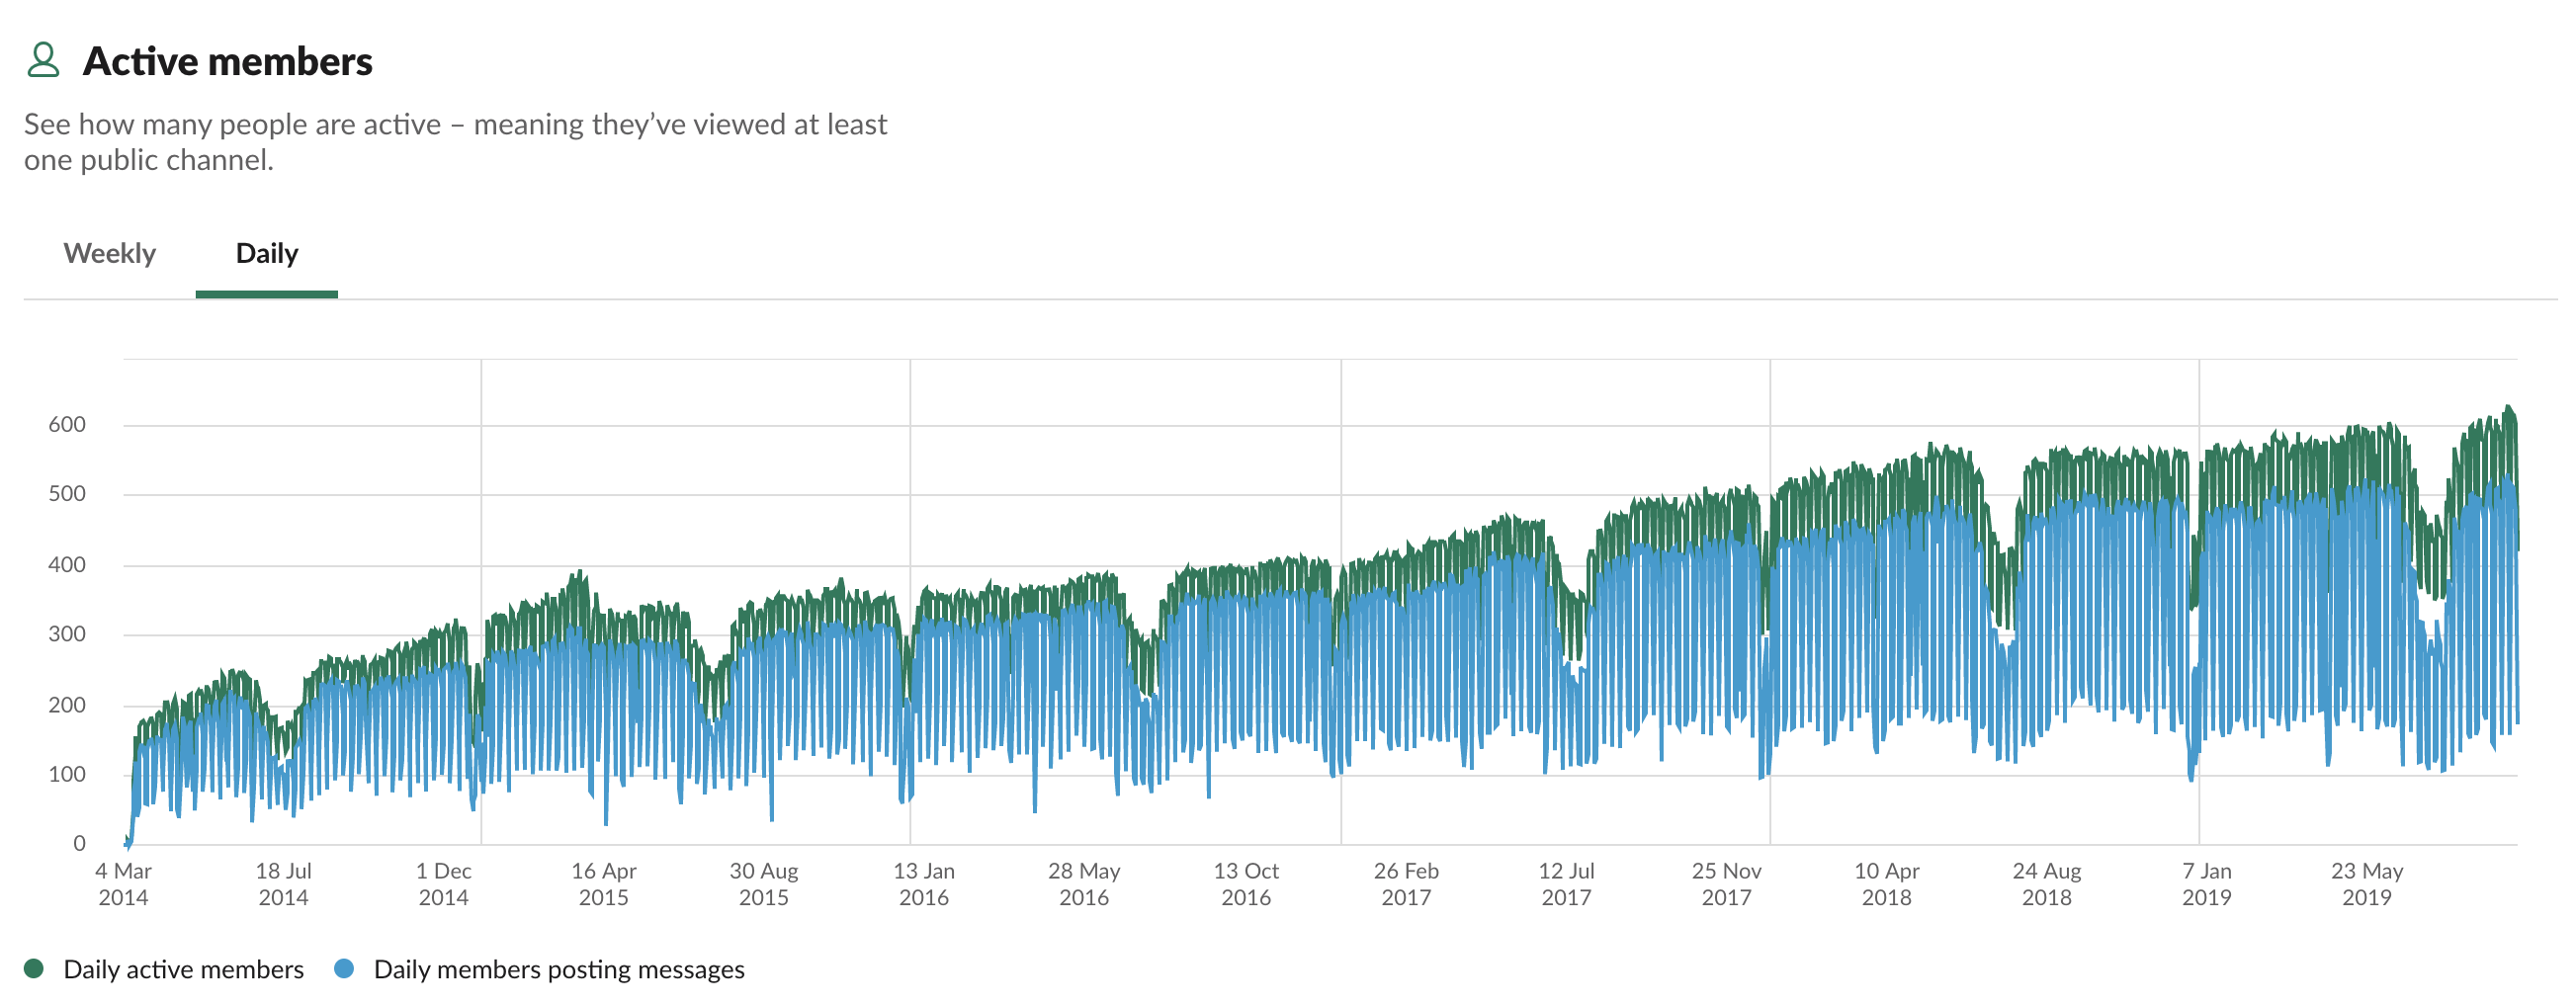
\includegraphics[width=1\textwidth]{daily-active-slack-members.png}
  \end{center}
  \label{figure:slack-members}
\end{figure}

By analyzing the company's Slack channel visualized in figure \ref{figure:slack-members}, it can be seen that people in the company are very active. However, by performing a quick search on the history of the chat's with the term "Developer Experience", only 62 results were found. In comparison 441 results was found when searching with the term "User Experience". However, it is worth to mention that a big chunk of the discussion is in Finnish.

\clearpage
\section{Results}

This section reports the different result of the research.
% TODO: add more explanation here

\subsection{Results of the Multivocal Literature Review} \label{section:result-of-mlr}

The Multivocal Literature Review (MLR) performed on the definition of DX resulted in interesting results that presented and reviewed in the following sections. The data points collected emerged during the analysis, and the more analysis was done the more interesting revelations were found.

There are two different research groups that research DX. A research group in Brazil has to a large extent researched the DX in the context of Mobile Software Ecosystems (MSECO). To these ecosystems belong mobile application development platforms as Android and iOS. Their approach to DX can however be seen as something applicable to all kinds of products and services that aim to create a better DX and improve on it. Another group of researchers in Finland have studied the mood of developers and its effects at varying levels of software development. To this group is also linked other studies related to the DX of IDEs.

% TODO: rename all occurrences of "scientific" to "white"?

\begin{table}[ht]
  \begin{center}
    \begin{tabular}{l | r r | r}
                        & \textbf{Scientific literature} & \textbf{Grey literature} &     \\
      \hline
      \textbf{Included} & 39                             & 19                       & 58  \\
      \textbf{Excluded} & 50                             & 2                        & 52  \\
      \hline
                        & 89                             & 21                       & 110
    \end{tabular}
    \captionsetup{width=0.6\textwidth}
    \caption{Number of sources analyzed for the MLR}
    \label{table:number-of-sources}
  \end{center}
\end{table}

\subsubsection{The object / entity of DX under study}

Based on the DX framework presented by \textcite{fagerholm-doctoral-thesis}, a data collection point was included to understand the object or entity under study of DX. This addresses the first research question, specifically \hyperref[RQ1.1]{RQ1.1}. The experience object is what is experienced in itself. This could be some artifact e.g. the IDE in the developer's development environment. However, it can also be something more abstract like the conventions or unwritten rules that a software team has established.

\subsubsubsection{Object under study in scientific literature}

In scientific literature the most prominent object under study was the \textit{usability} of various objects e.g. the IDE and API. This stems most likely from the fact that DX is seen as a variation or extension of UX. In many articles the definition of developer experience is related to or derived from UX. Usability of developer tools, programming languages, and APIs are concrete, important, and measurable examples of objects of DX. DX is however not limited to UX of tools and services.

Other emerged objects of DX under study in scientific literature included \textit{the support for developers, technical environment, developer's activities in a community, wellbeing of developers, and individual developers in a bigger context}.

\textit{Support for developers} was addressed by discussing about frameworks that support developers in their daily development activities. This includes development practices, processes, and guidelines that aid developers in developing software. Support is not only limited to technical procedures, but includes also emotional and social support. This emotional aspect of DX is visible in other places and is not limited to support for developers.

\textit{Technical environment} or the development infrastructure is concrete example of an object under study. The technical environment includes the development products and services and other tools that developers use to create and develop software. The most studied tool that developers use was the IDE or code editor. The reason behind this is not known, but one possible reason is that developers spend a big part of their time reading and editing code. Therefore also the DX of the technical environment is getting attention in the studies.

\textit{Developer's activities in a community} relates to the activities a developer has in a community of other developers. Development is a social activity, that often is performed in conjunction with other developers in a team. Developers create communities on different levels that can be very local e.g. a single software team

\textit{Wellbeing of developers} was discussed in multiple articles. Mainly this was a discussion topic of the research group studying the happiness and unhappiness of developers \parencite{what-happens-when-unhappy}, \parencite{unhappy-developers}, \parencite{consequences-of-unhappiness}, \parencite{on-the-unhappiness}. They focus mostly on the happy-productive theory of developers. This set of studies and research focuses mostly on the happy-productive theory of developer, but there can also be seen a general interest towards the wellbeing of developers.

\textit{Individual developers in a bigger context} was not a self-evident object under study. \textcite{entering-an-ecosystem} and \textcite{fagerholm2014examining} were the two most obvious studies of this aspect of DX. However, this can also be found from other objects under study, sometimes directly but mostly more indirectly.

Further iterating on the emerged objects / entities under study, it became more clear that the underlying object under study was the developers' point of view as in \textcite{voice-of-the-developer}. In the past decision relating to software tools or other used techniques and procedures were made by managers and directors. Today there can be seen a trend that has turned the tides, and given developers more decision power when creating and developing their own ways of working. In general there is an interest towards supporting developers and their daily activities in the environment they are working in. The wellbeing of developers is seen important and different viewpoints on how this can be improved

\subsubsubsection{Object under study in grey literature}

The first iteration of the grey literature and its objects under study revealed categories as \textit{starting experience, API DX, developer portals, usability, developer developing for other developers, developer tools, developer support, development platforms}. Most obvious object under study were APIs, their usability and the necessities around the APIs.

\textit{Starting experience} was found in one grey literature article, and it captured an important object of DX. Developers are constantly learning new stuff and adopting new technologies and techniques. The starting experience of new tools, products, and services is in a crucial role when developers pick their selections for upcoming projects and products. The starting experience was also called \textit{"0 to 200"} and \textit{"Time to Hello World"}.

\textit{API DX} seems also to be a hot topic in the industry. There has been lately discussions about a new term called \textit{API Economy} \textcite{web-api-economy}. APIs have become important assets for companies, and some companies are even relying their whole businesses on to providing APIs. Developers are the main users of APIs and therefore the API's UX and DX are important for the business. DX in the context of API is mostly usability, but includes also other aspects like the starting experience, documentation, and adoptability.

\textit{Developer portals} are websites and documentation libraries where developers can find information and examples about products and services aimed towards developer, mostly APIs. The portals can include and overview of the service's different functionalities, specifications and guidelines. The gist of developer portals is to allow developers to make well informed decisions.

\textit{Developers developing for other developers} makes DX different than UX. In many articles in grey literature there were given guidelines on how to create a good DX of a software library or tool. The open source movement and community is a good example of where a developer develops for another developer. Developers are technical and therefore there is also a risk that their libraries and products that they write become too complex and unintuitive to use. Popular software libraries and frameworks are putting effort into creating a good DX, that will benefit the developers using them.

\textit{Developer support} continues on the category of developers developing for other developers. The category is vague, but in the literature there were discussions about topics like developer relations and support provided by communities. One article discussed about sympathy and empathy towards developers, and how the lack of it can be harmful for the DX.

\textit{Development platforms} did also get attention in the grey literature. Different development platforms are competing of developers. For example, in the mobile software development context, the main two platforms iOS and Android are "competing" against each other for developers. One way these platforms can gain more developers and build communities is by creating and maintaining a good DX.

As a conclusion we can see that the objects of study of DX in grey literature is more focused on the practical and technical parts of DX. And because most of the found grey literature articles were blog posts, they were focusing on the business of products and services. This caused that the most discussion revolved around usability and technical aspects of DX.

\subsubsubsection{Comparison between scientific literature and grey literature in the object of study of DX}

There is a lot of similarities between the scientific and grey literature regarding the object under study. Usability was the most occurring object of study in both of them. The technical environment was also clear on both sides.

Scientific articles were dwelling more equally on cognitive, affective, and conative, the 3 aspects of DX while grey literature was clearly more focusing on the cognitive parts of DX. Scientific literature was also focusing more on the feelings and moods of developers, while only a small part of the grey literature focused on this.

\subsubsection{Factors that improve or worsen the DX}

What improves and/or worsens the DX as in \textcite{fagerholm-doctoral-thesis} was also included in the data collection form. When understanding the object of DX, there is also something that improves or worsens the experience, i.e. what influences the experience. The discovered factors were no direct statements found in the sources, but were factors that emerged when analyzing the articles as a more coherent set of articles.

\subsubsubsection{Factors that improve/worsen the DX found in scientific literature}

Notable factors in scientific literature that improve DX were many, including \textit{shared understanding,	available support, collaboration, expectations, mitigating complexity, being in control, ability to tackle challenges, having a meaning as a developer, guidelines, information availability}.

\textit{Shared understanding} was mostly discussed in the articles discussing Performance Alignment Work \parencite{paw}, \parencite{how-developers-experience-team-performance}. However, this pattern can be found in most of the articles. Having a shared understanding between developers, but also with other stakeholders seems to improve DX.

\textit{Collaboration} and the benefits that are achieved from working together improves DX. Getting quick feedback from teammates, having agreed policies and roles but being flexible and agile all improve the experience developers have when collaborating with others. \textcite{entering-an-ecosystem} studied the different systems surrounding a developer in a open source community

\textit{Mitigating complexity} and simplifying things was mentioned explicitly in some articles, but was also apparent in many other articles implicitly. Developers are solving difficult technical problems in complex domains. Developers have to understand both the technical opportunities and constraints, but they also need to understand the business value of what they are doing. This means that developers have a lot on their mind, and therefore all complexity might affect developers DX negatively.

\textit{Being in control} relates to the developers feeling that they are in control of what they are doing. Overwhelming situations were developers feel that they are not in control might worsen their DX. Here the selection of tools also plays a role. The perceived selection of tools affects also the developer DX \parencite{software-developers-as-users}. Throughout the years there has been a shift in selection of tools, that has more leaned towards developers. Reaching a flow state is also an important part of feeling of being in control. Achieving a flow state shows that external and internal distractions of developers are minimal, and that developers can focus on the essential, developing. Uncertain situations was

\textit{Ability to tackle challenges}. Challenges are inevitable when developing software. However, the ability to tackle them was seen as a factor that improves DX. \textcite{what-happens-when-unhappy} concluded that being stuck in problem solving affects significantly developers' mood and happiness. These problems can be anything relating to development practices like difficulties with a framework or library, algorithm logic, IDE, other development tools, deployment of software, maintenance, etc. The ability to tackle challenges relates also to the before mentioned factor "being in control".

\textit{Having a meaning as a developer} and having explicit and aligned values within the team and organization improves the motivation of developers, and presumably also the DX. Aligned values can relate to the product and its goals, but also to teammates and their goals. \textcite{fagerholm2014examining} concluded being able to put the value system of a team into words is more important than the methodologies. This can help with understanding what the team is aiming for and what the goals of the team is. Developers that understand the values, and possibly also share them with others might have a greater sense of meaning regarding their development tasks.

\textit{Information, guidelines, and support} was the most obvious emerged factor that improves DX. Developers are constantly in a learning process, and for example the information, guidelines, support, code examples, and instructions affects the developers DX significantly. Availability, quality, and relevance of all these are important as developers time is limited. The time between getting stuck in problem solving and finding a solution and way out is minimized with good support for developers.

All the combined scientific factors that improve DX shows that DX is improved by mostly affective and conative aspects. This includes the feelings and perceptions of developers. Even if the studied articles were mostly discussing about cognitive aspects like tools and processes, and especially usability, there is the common pattern that developers own feeling and perceptions is what creates a good DX.

\subsubsubsection{Factors that improve/worsen the DX found in grey literature}

The most significant factor that improves DX was the UX and usability of tools. Usability of APIs, tools, and products all affect the DX. These usability factors include esthetics, exclusivity, fun, completeness, functionality, experience, pleasure, and reliability. When further analyzing the grey literature, factors as \textit{transparency towards developers,	explicit guidelines, developers loving their tools, sympathy, feeling of capability, developers are human too, support towards the development process} emerged.

\textit{Transparency} was one of the indirect factors that emerged in the grey literature. Transparency means in this context the transparency of the development artifacts that developers interact with in their daily work. One example of transparency could be the running application in the production environment, where the state and the possible errors are available to the developer. Another example, that was not apparent in the literature, could be the transparency of the whole organization where the developer works. Developers that have a honest and clear understanding of the whole organization that they are working in, will probably have a better DX.

\textit{Explicit guidelines} of tools, products, and APIs reduces the complexity and by that also improves the DX. All kinds of communication like documentation, guides, and examples were factors that contribute to the DX.

\textit{Developers using tools they love} was an interesting factors found out in one of the articles in grey literature. Developers are spending most of their work time with the development tools, and therefore it is regarding their DX important that they show affection towards them. The perceived choice of developers when selecting tools, and concluded that if developers are able to make their selection themselves, they are going have a significantly better DX.

\textit{Sympathy} was mentioned as improving DX in one specific article in the grey literature. However, sympathy can be seen in all the other factors as well. Different roles in software team that understand each other, create an experience that is also affecting the DX.

\textit{Feeling of capability} emerged as an factor and developers need to have the feeling of that they are capable of solving the problems they face to have a good DX. An empowering environment increases the motivation of developers to solve problems.

\textit{Developers are human too} was a title of one of the titles in the grey literature, and seemed to also be a notable factors when understanding what improves the DX. The phrase "developers are human too" indicates that there might have been a lack of understanding towards developers, that should be changed. Interestingly some articles were also discussing about how developers hate marketers, and that they want to make their tool buy-ins based on facts and experiences, and not by material produced with the aim of selling products. This shows that developers are aware of that they might not get the treatment that they deserve, and that the developers know that they are not just a resource or object utilized by software development organizations.

\textit{Support towards the development process} was identified to contribute to a better DX. Supporting the development process, like improving tools and services. For example, the management showing their support and allocating resources to improving the development process could improve the DX.

\subsubsubsection{Comparison of scentific and grey literature of factors that improve/worsen DX}

UX and usability of tools, APIs and products is the most obvious factor that improves DX. This is probably because that is the most easy and tangible definition and measurement of DX.  Further analysing the results however shows that there is more of what impacts the DX. In both scientific and grey literature there was the underlying factor of \textit{"feeling of being capable"} that improves the DX. This was also in line with \textit{"being in control"} that was also found. These both categories touch on how the developer sees their own work.

\subsubsection{Research methods that have been used to study DX}

A list of research methods used to study DX can be found in table \ref{table:research-methods}. From the nature of the research topic in the studies, it is apparent that most of the research methods are exploratory in nature.

\begin{table}[ht]
  \begin{center}
    \begin{tabular}{l}
      \hline
      Interviews                              \\
      Survey                                  \\
      Literature review / Systematic mapping  \\
      Study of related approaches             \\
      Trainings / Experiments / Diary studies \\
      Design research                         \\
      Case study                              \\
      Expert experience                       \\
      Repository mining                       \\
      \hline
    \end{tabular}
    \captionsetup{width=0.6\textwidth}
    \caption{Different research methods used in studying Developer Experience}
    \label{table:research-methods}
  \end{center}
\end{table}

\subsubsubsection{Research methods in the scientific literature}

\begin{figure}[ht]
  \captionsetup{width=0.6\textwidth}
  \caption{Research methods of Developer Experience in scientific literature}
  \begin{center}
    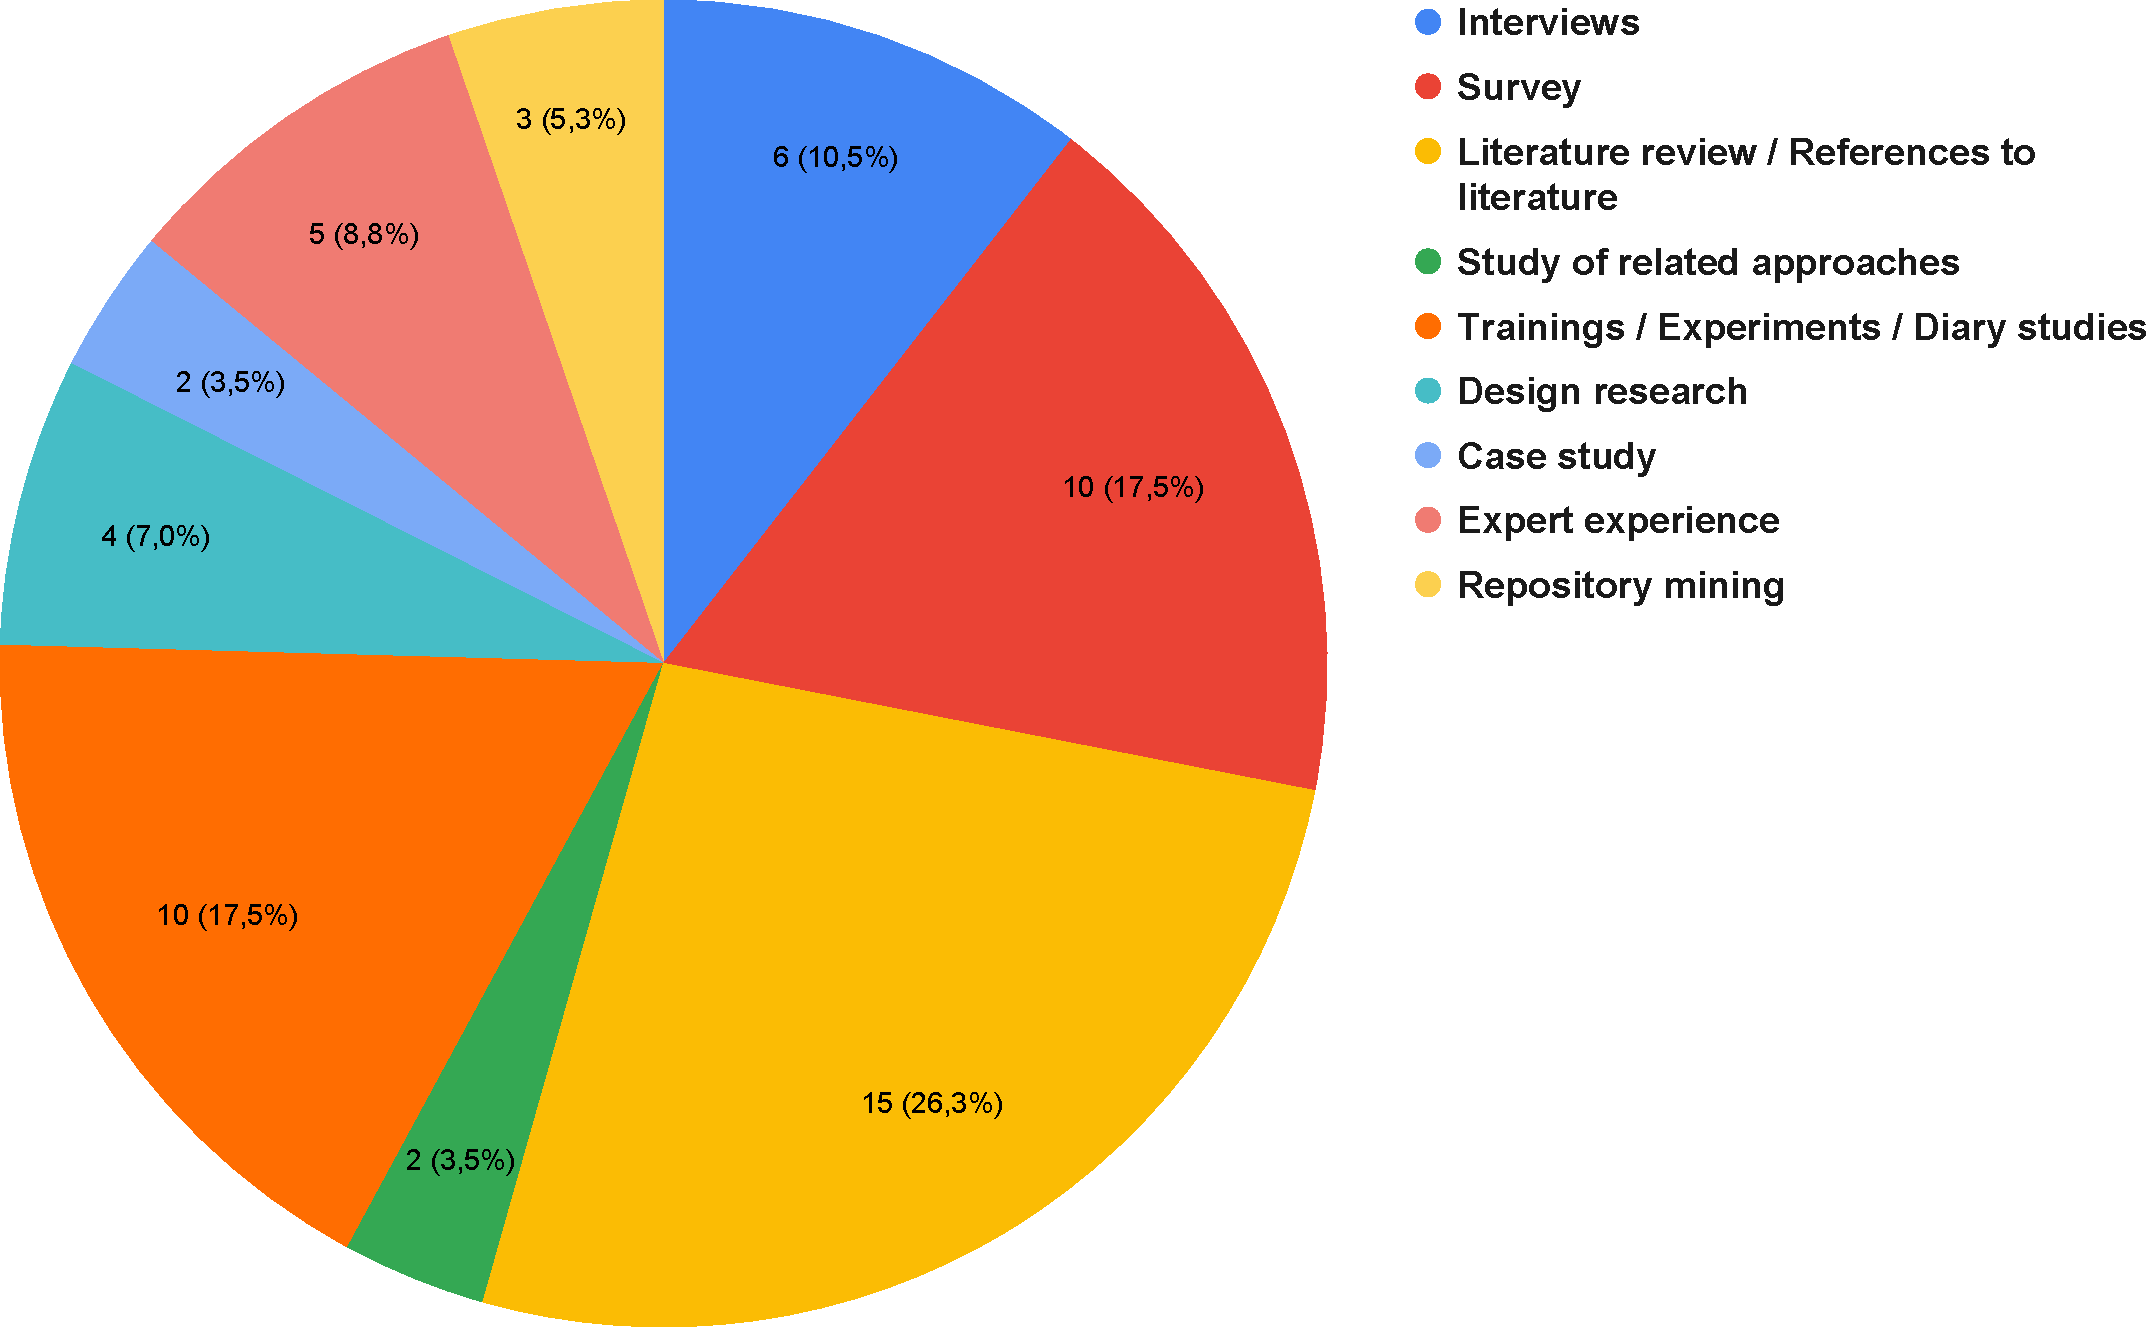
\includegraphics[width=\textwidth]{research-methods-scientific.pdf}
  \end{center}
\end{figure}

Mostly the results of the studies were based on literature review and some qualitative methods like interviews, surveys, and diary studies. There were also some design science researches and case studies. Case studies and research designs are probably popular because they provide academics a way to collaborate with practitioners. This is common especially in software engineering, as the industry might be leading the way ahead the academic research.

Some data repository mining was also performed to find out patterns in developer behaviour. This type of research is interesting and had been enabled by the large developer communities that provide opportunities for data mining and analysis. Examples of these are StackOverflow and GitHub.

Experiments, trainings and observational studies were also a common research method. These were utilized in studies were the focus was on different objects of  was on the usability of  like the IDE or the programming language utilized control groups and experiments.

\subsubsubsection{Research methods in the grey literature}

\begin{figure}[ht]
  \captionsetup{width=0.6\textwidth}
  \begin{center}
    \caption{Research methods of Developer Experience in grey literature}
    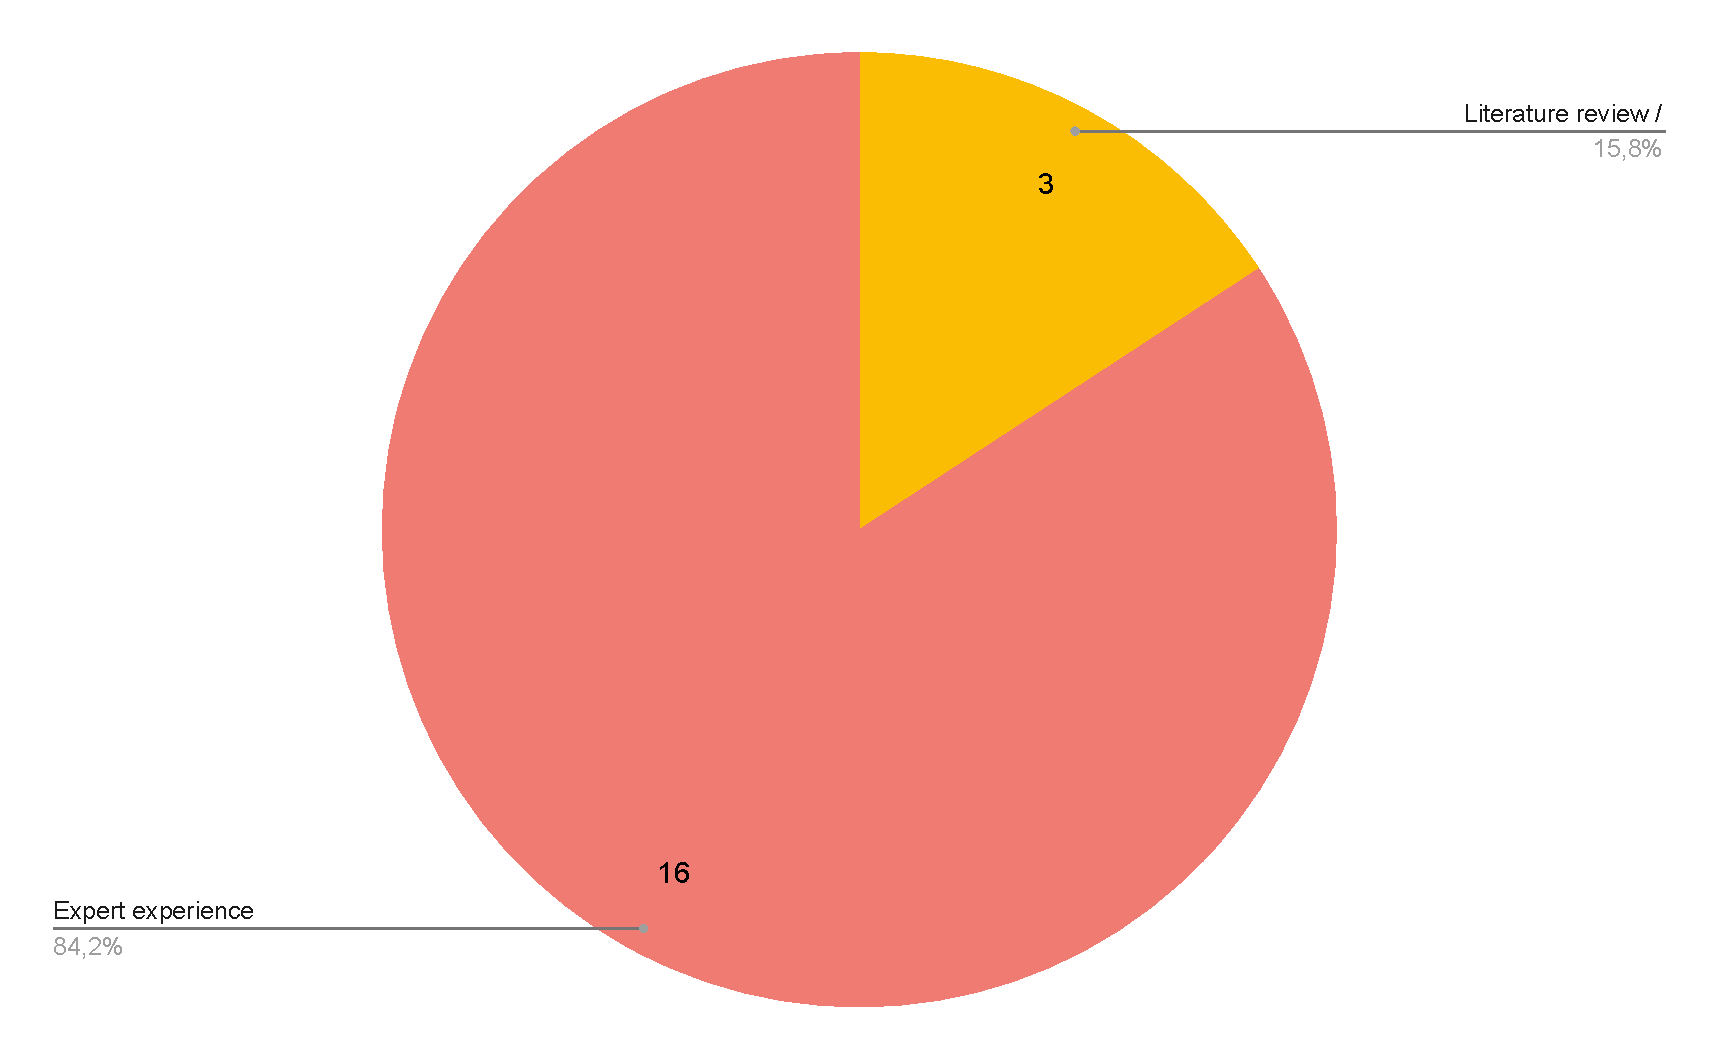
\includegraphics[width=\textwidth]{research-methods-grey.pdf}
  \end{center}
\end{figure}

In the grey literature the research methods are all expert experience reports where practitioners from the industry report their experiences and lessons from them on blogs and other websites. However, the grey literature articles were quite heavy in references, where the authors were used either someone else's writing or their own writing to base their statements.

\subsubsection{Explicit / implicit definition of DX}

Interestingly, during the analysis of the sources, it emerged that some articles were stating an explicit definition of DX, but some were not. To analyze how the the definition of DX is given, all articles and papers were grouped into either having an \textbf{implicit} or an \textbf{explicit} definition of DX. This division was something that did emerge in the collection and analysis of the material. Many scientific articles use the keyword "developer experience", but only mention DX briefly in their material. This forces the readers to create an understanding of what DX, and "read between the lines" while acquiring the gist of the articles.

\textit{Explicit definition} of DX means that the author has in some words explained or defined the concept of DX, or referenced some other material that gives the definition to it. \textit{Implicit definition} of DX means that the author doesn't give any definition or explanation of what DX is. The definition can often however be inferred from the context of the paper.

\begin{figure}[ht]
  \captionsetup{width=0.6\textwidth}
  \caption{Implicit vs. explicit definition of Developer Experience in scientific literature}
  \begin{center}
    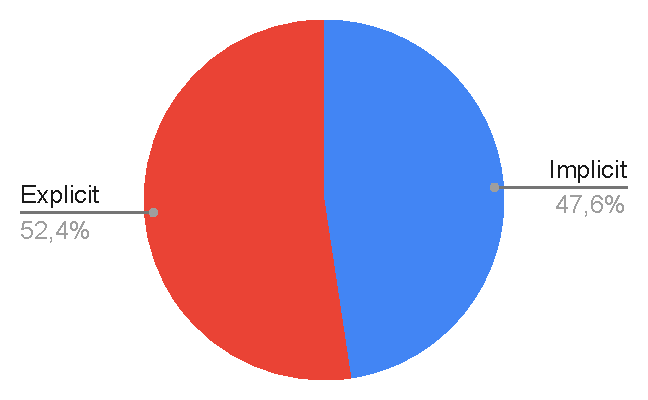
\includegraphics[width=0.6\textwidth]{definition-scientific.pdf}
  \end{center}
\end{figure}

Scientific papers are almost equal in both giving an implicit or explicit definition of DX. It shows and confirms that DX is an topic and research area that has not gotten much attention at the moment of writing. Some research areas have been developed so far that there is things that can be taken for granted. However, the are of DX might not yet be at that point yet and therefore

\begin{figure}[ht]
  \captionsetup{width=0.6\textwidth}
  \begin{center}
    \caption{Implicit vs. explicit definition of Developer Experience in grey literature}
    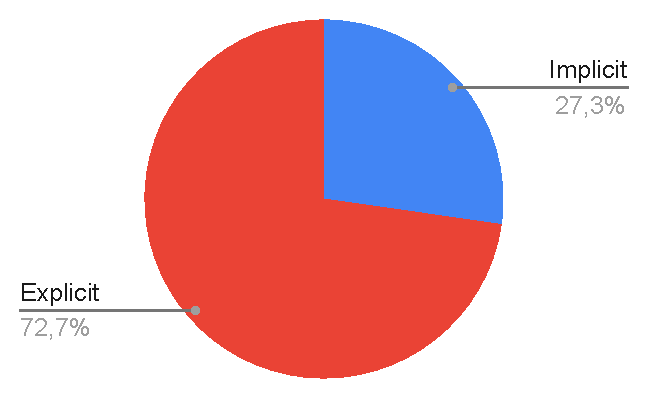
\includegraphics[width=0.6\textwidth]{definition-grey.pdf}
  \end{center}
\end{figure}

Grey literature has a majority of explicit definition of DX. The articles are often starting with giving an explanation of their viewpoint and definition of DX. Quickly the articles then continue to discuss the topic from the selected context and viewpoint.

\subsubsection{Context of DX}

From the analysis of the material, there is a clear indication that there are different viewpoints and contexts to DX. The different contexts that emerged from the analysis are listed in table \ref{table:contexts}. The context were completely unknown before starting the MLR. One source address the topic of DX from multiple contexts and viewpoints.

\begin{table}[ht]
  \begin{center}
    \begin{tabular}{l}
      \hline
      Definition                        \\
      Development Environment           \\
      API                               \\
      Product or service                \\
      User Experience                   \\
      Team, Collaboration, \& Community \\
      Knowledge sharing                 \\
      Mood \& Feelings                  \\
      \hline
    \end{tabular}
    \captionsetup{width=0.6\textwidth}
    \caption{Different contexts of Developer Experience that emerged during the literature review}
    \label{table:contexts}
  \end{center}
\end{table}

\textit{Definition} is the context that considers directly the definition of DX. Articles having the context of definition are discussing and explaining the concept of DX. They either implicitly or explicitly add to the definition of DX, either from their own point of view or then from a more broader context.

\textit{Development Environment} is related to the technical environment where the developer is developing the software. In the found articles the most notable artifact under research was the IDE. Other artifacts that could be included in the development environment could be programming languages and framework or the ease of use of setting up the development environment.

\textit{APIs} emerged as a context. APIs are interfaces that developers use when building software. This makes developers users of the APIs, and their UX of an API can formulated to be a DX.

\textit{Product or service} is related to the APIs, but was selected as a separate context. Software developers use products and services to develop software, and was seen as an important context of DX. The grey literature is heavily influenced by businesses marketing their services or products. To gain visibility and recognition, businesses are publishing articles and posts on their blogs to write and discuss a specific topic. These businesses are defining DX from their own point of view where they are providing products and services, that are directly used by developers. Some articles mentioned that back in the days, it was executives that made the business and purchase decisions of tools, frameworks and other products and the developer's opinion were not considered. Developers were forced to use whatever they were offered. Today, the purchase decision has more and more shifted to be a responsibility of the developer. Developers are the final users of the product and therefore businesses have probably realized that developers are the ones to make the decisions. All in all, it can be seen from the current grey literature that developers are being considered more and more (cite "Devs are people too"), and that this movement has created the concept of DX.

\textit{User Experience} is the experience that emerges from using a software product or service. Multiple sources explained that DX is a form of UX. Grey literature takes to a large degree a viewpoint where DX is a form of UX, where developers are users of products and services. In this viewpoint the DX consists of features that are also used when measuring the UX of a service. These include factors like functionality, usability, and reliability. DX can be seen that there is always a developer that is a user. The role of the user is the variable, and can vary from being a user of a product where the DX is seen in the product, or then the user can be a user of a developer workflow in a software project.

\textit{Team, Collaboration, \& Community} was seen as a specific context that includes the social aspect of DX. Multiple sources discussed about the team and communities where software is developed. They were considered to have a great impact on the DX. The scientific research is more focused on the social parts of DX, and scientific research has taken a step further in this than the grey literature.

\textit{Mood \& Feelings} emerged from the multiple articles discussing the happiness of developers. The mood and feelings should not only be restricted to happiness and/or unhappiness. DX allows developers to reason about things that before has been difficult. Making statements that are in the favour of developers might have been difficult as there hasn't been any term to coin the feelings, emotions, needs, and desires.

\begin{figure}[ht]
  \caption{Context of Developer Experience in scientific literature}
  \begin{center}
    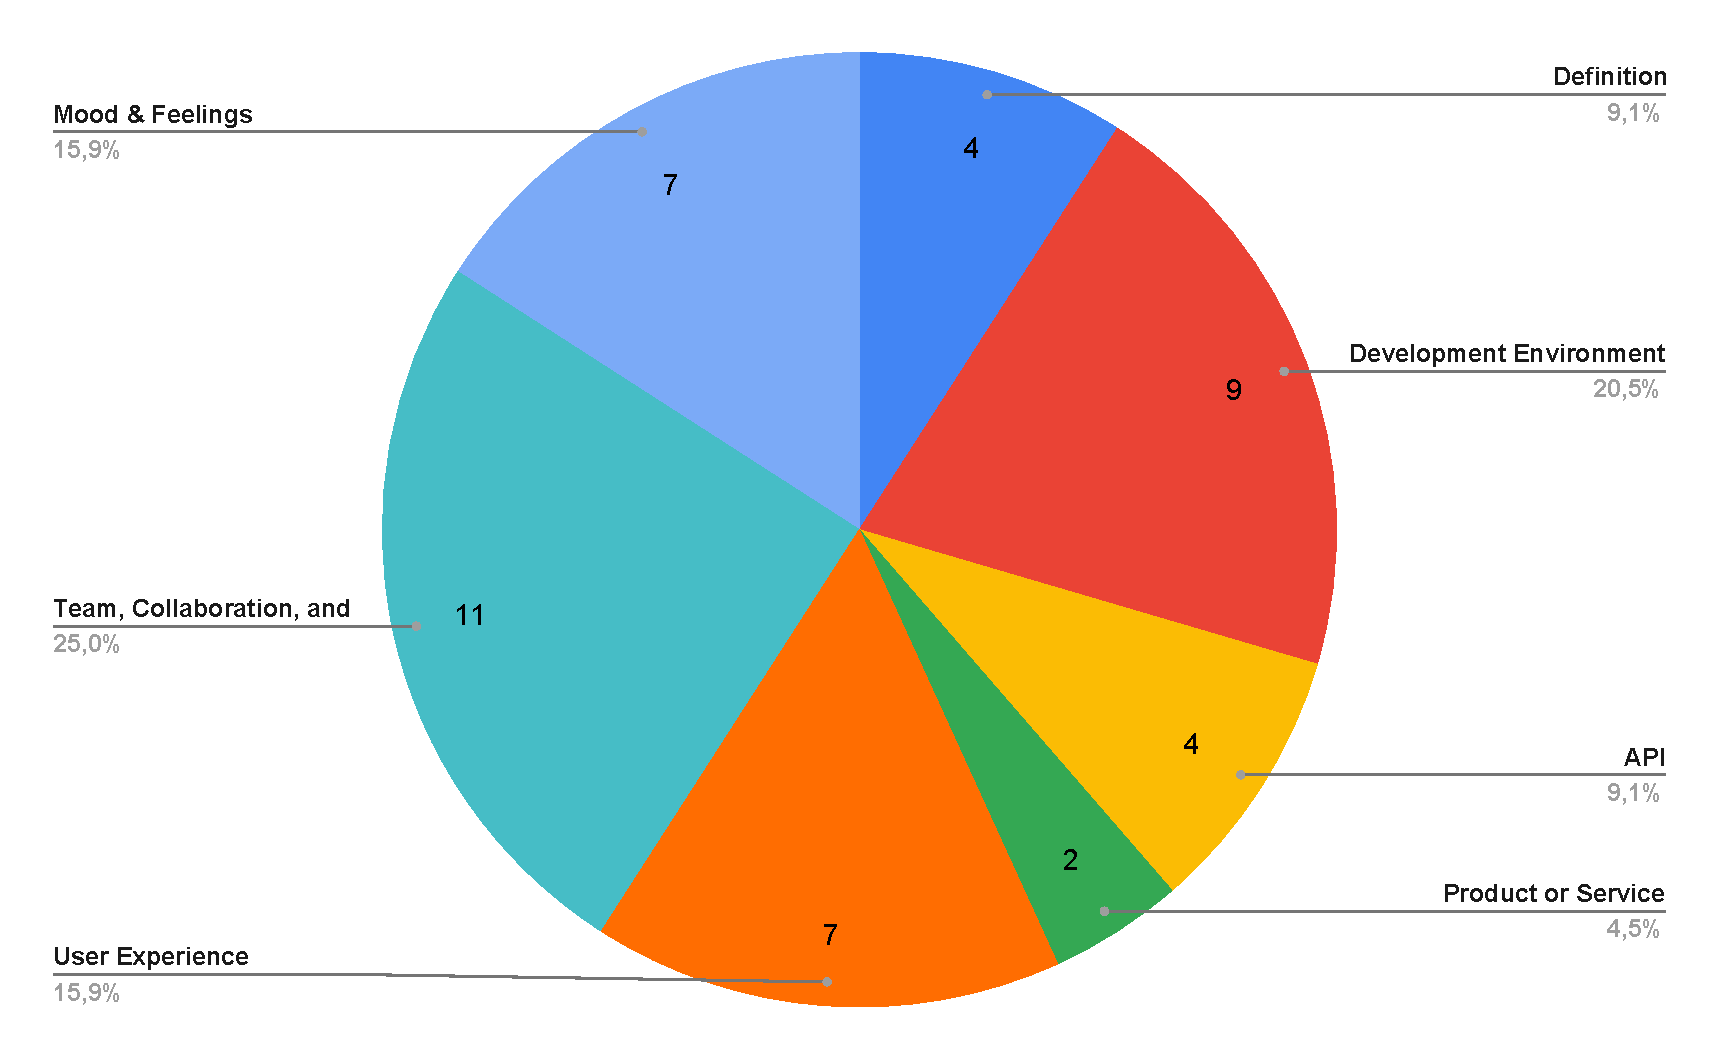
\includegraphics[width=\textwidth]{context-scientific.pdf}
  \end{center}
\end{figure}

\begin{figure}[ht]
  \caption{Context of Developer Experience in grey literature}
  \begin{center}
    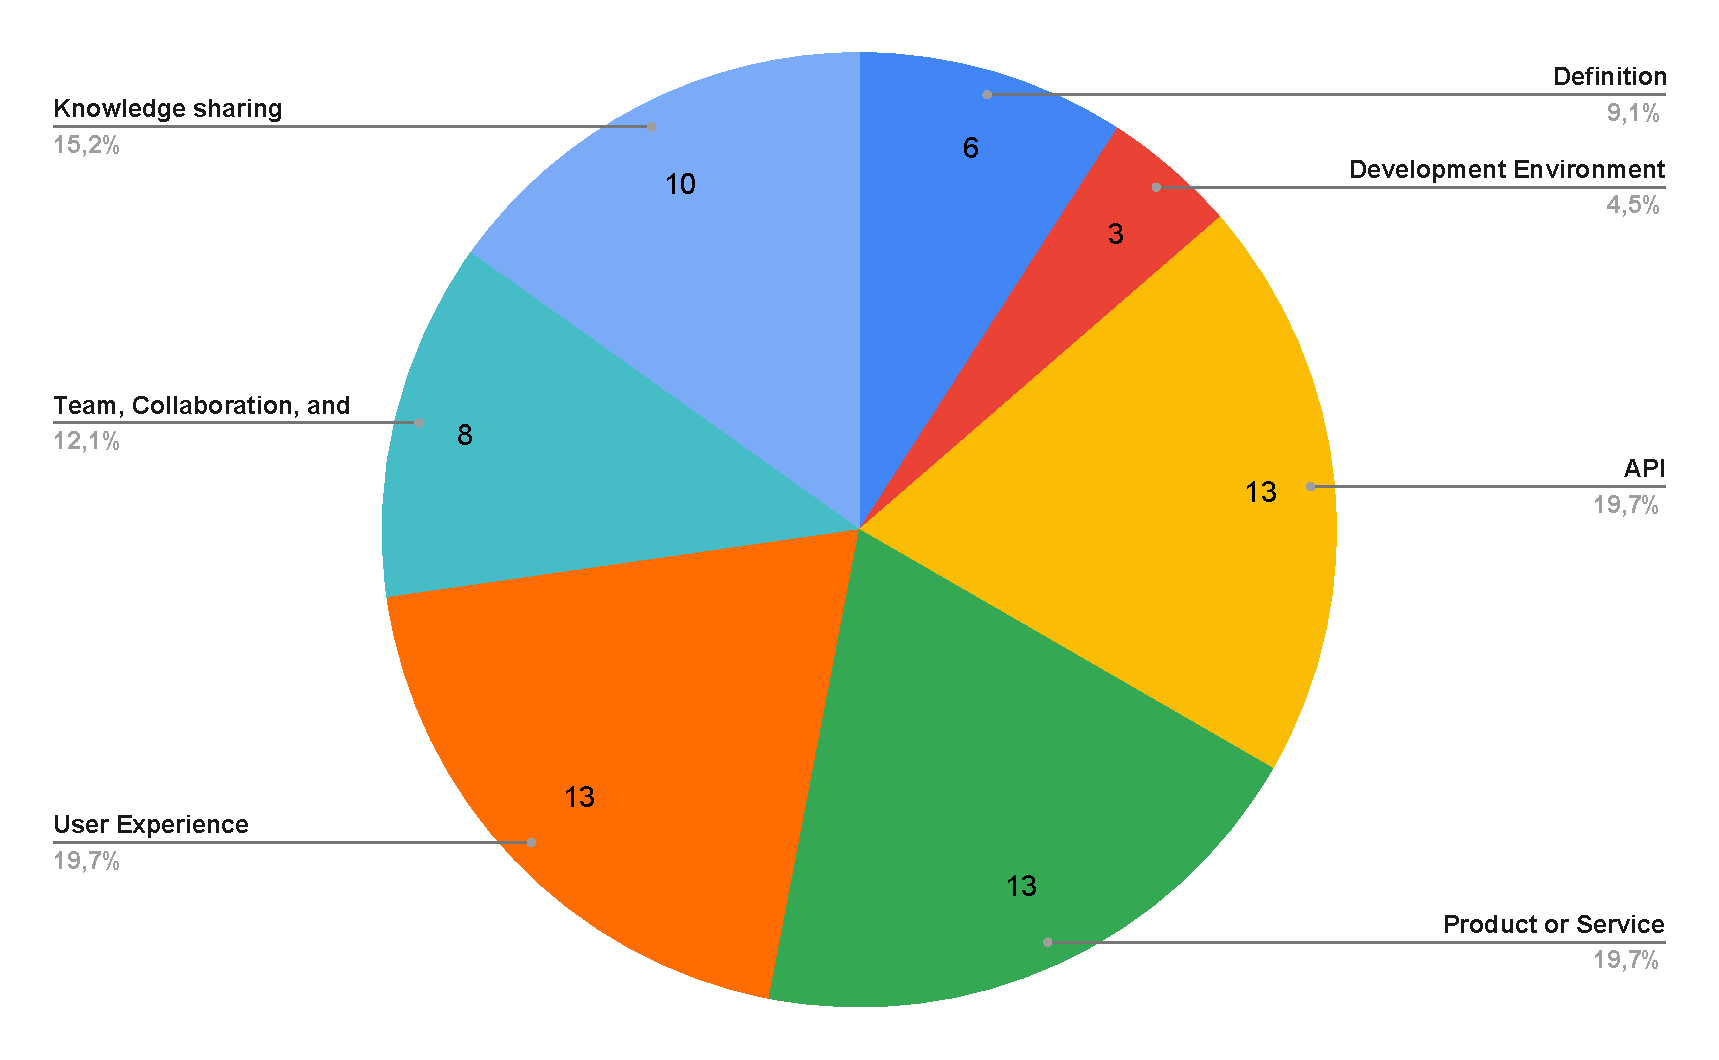
\includegraphics[width=\textwidth]{context-grey.pdf}
  \end{center}
\end{figure}

\subsubsection{Categories of definitions of DX}

To summarize the analysis of what the studied objects of DX are, what the factors that improve/worsen the DX are, the explicit and implicit definitions of DX, and the context of from where DX is looked from, and attempt to understand the definition of DX was made. This was also a data point in the data collection form, and each article's short definition of DX was added to the form. The subsequent sections analyze the definitions on both the scientific and grey literature.

\subsubsubsection{Categories of definitions of DX in scientific literature}

The most common definition of DX used in the scientific papers is the concept and definition presented by \textcite{fagerholm-dx-concept-and-definition} and \textcite{fagerholm-doctoral-thesis}. This definition is at the moment of writing (\now) the only explicit attempt and deep dive into giving a definition of DX in the scientific literature. There is also further derivations on this concept and definition, but nothing that is refuting their definition and concept or nothing that takes another viewpoint on the definition of DX.

The definition given by \textcite{fagerholm-dx-concept-and-definition} was apparent when looking at results of the analysis of the definition of DX in scientific literature. The most apparent and noted definition of DX was \textit{developers thoughts and feelings towards their work}. The thoughts and feelings included subjects as the mood of developers, working environments, social aspects, processes, and basically anything that relates to the daily work activities that developers are conducting. Other categories of definitions were \textit{activities, technology, usability, values, agility combined with the starting experience, and expectations}.

\textit{Activities} refer to the all the different activities, and the experiences of them, of a developer. In the literature these activities are defined as anything that the developer encounters in their software development tasks. A good example of a definition of DX regarding activities was

\begin{quotation}
  \noindent \textit{"Developer Experience relates to all kinds of artifacts and activities that a developer may encounter as part of his/her involvement in software development"} (\textcite{ekwoge2017tester} based on \textcite{fagerholm-dx-concept-and-definition})
\end{quotation}

\noindent \textit{Technology} was another, quite broad, category of definition that was found.  Almost all articles discuss about the technologies that developers use, and that they are a main contributor to the definition of DX. In e.g. \textcite{nebeling2013informing}, measurement of the DX of different mobile development platforms was performed by grading the platforms from the point of view of the technical (e.g. programming language, IDE, debugging tools), subjective (feelings towards the platform), and the level of productivity (ratio of output vs. effort). However, for example, \textcite{silva-comparing} took an exclusively technical viewpoint on the definition of DX, and could be loosely interpreted to be defined as \textit{as the ability to construct models with help of visual modeling languages}.

\textit{Usability} and UX was seen as being part of DX, and one definition of DX falling into this category was \textit{"UX characteristics of an IDE in the developers development environment"} \parencite{software-developers-as-users}. The other definitions found in this category are also related to this definition, the UX and usability of any artifact in the software development activities.

\textit{Aligned values} of developers and the bigger organizations that they are working in captured the different definitions were the DX is defined as the set of values, and their alignment with bigger entities of the software development process. \parencite{fagerholm2014examining} state that \textit{developer experience is formed in the value system of the development environment, both individually and in groups}.

The definition of the selected sources for the majority follow the definition grounded by \textcite{fagerholm-doctoral-thesis}. Almost all sources take some approach to DX, either cognitive, affective, or conative. This is especially true in the scientific articles, where there are more comprehensive groundwork done on why the research in question is performed.

\subsubsubsection{Categories of definitions of DX in grey literature}

In grey literature the definition of DX varies a lot more and there are no references to any scientific sources in the grey literature. The definitions are given by the practitioners themselves and from their viewpoint and context of software engineering. In many of the grey literature articles the authors have their own view and definition of what DX is. Only in few articles there is actual questioning of the definition of DX. During the analysis there were 4 different categories of definitions of DX that emerged. These include \textit{the experience of using a software product, understanding the developer, experience from idea to code to delivering business value}, and finally \textit{support and help for developers}.

\textit{The experience of using a software product} was interpreted as the definition of DX in multiple articles.

\begin{quote}
  "Developer Experience (DX) is the equivalent of User Experience (UX) when it comes to a developer" \parencite{the-best-practices-for-a-great-dx}
\end{quote}

\noindent The category of \textit{understanding the developer} consisted of the following definition:

\begin{quote}
  "DX design is about understanding the context of use, understanding what developers need to complete their tasks, underlying technology, integration points, and focussing on how developers feel while using a product or services." \parencite{building-the-developer-experience-from-the-ground-up}.
\end{quote}

\noindent There seems to be a consensus that understanding the developer is important when creating a good developer experience.

\textit{Experience from idea to code to delivering business value} was a category that was created from a quote in \textcite{workflows-for-the-new-developer-experience} where they write about a talk on platforms and DX of them. This category included also viewpoints on the starting experience, and about how developers understand what is possible and what is not.

\textit{Support and help for developers} was the final category of definitions in grey literature. This category had definitions that focused on making the developers life as easy as possible, and about creating a seamless experience for developers. Improving and optimizing how developer get their work done allows to create a better DX. This category emerged from the articles that discussed about third party library, framework, and tool authors (developers) that have other developers as their users or customers.

\begin{quote}
  "... Developer Experience (DX) — which is all about using User Experience (UX) techniques to make life easier for third-party developers calling your public APIs ..." \parencite{4-must-read-articles-on-developer-experience}
\end{quote}

\subsubsubsection{Difference between the definition of DX in scientific and grey literature}

There can be seen both differences and similarities between the definitions of DX.
% TODO: more here

\subsubsection{Conclusions of the sources}

The articles report that DX is an important factor of software engineering. From the different contexts emerged in this study it is apparent that DX can be seen from a wide variety of different viewpoints. The different data points that were collected showed interesting results about the different aspects of DX, both in scientific and grey literature. There were both similarities and differences between them.

One main finding from the MLR, that applies for both scientific and grey literature, is that in software engineering in general there has happened a change in the empathy and sympathy shown and expressed towards developers. Almost all articles analyzed were discussing about DX in a humane and compassionate tone. This is also noted in \textcite{voice-of-the-developer}. However, there is still a lot of "objectifying" of developers the same way as there might have been towards users of the early stages of HCI and before user-centered design.

\subsection{Validity of results}

\subsubsection{MLR}

The search engine Google is known to provide results based on many different variables on the user e.g. previous searchers, internet profile etc. Therefore the search results from Google might not present results that are applicable for anyone. To mitigate this, private browsing sessions were used on the browser when performing the searches.

Google has not revealed how the search engine optimization (SEO) works on the Google search engine. However there are some broad guidelines on what a web page has to include, so that it will rank higher on the results page. For companies Google search results is a huge asset and a big opportunity to gain visitor traffic and publicity. Having a web page or site ranking high on the Google search results can probably even determine the existence of some companies businesses. All in all, this means that ranking high on the Google search results page requires knowledge and effort. Therefore we can deduce that the grey literature resources included in this MLR retrieved from Google search are funded or backed by companies that deliberately aim for high ranking on Google searches to sell or promote their products or services.

Depth of data collection has probably varied while performing the MLR. In most cases no explicit analysis was required to extract the required data when collecting it. However, based on the quality of the source sometimes the collection required some analysis to be able extract the data. E.g. understanding the object of DX under study forced sometimes the researcher to "read between the lines", adding their own interpretation and possible bias to the data. This same problem was present also if the research topic of the source was not explicitly  studying DX, but still related to concepts of DX.

\clearpage
\section{Discussion}

Developer experience is an umbrella term that captures a big part how developers feel and perceive their work. Current definition of DX in the industry is largely based on practitioners own experiences. In academic writings and papers, the topic of DX is studied relatively little, and the existing articles are not well known by the research community.

Surprisingly the most used research method in scientific articles was literature reviews and systematic mappings. Even if the topic is novel and there is not much studies on it, the studies are basing their findings on previous work. One explanation to this could that DX is an umbrella term (hypernym) of multiple different hyponyms, e.g. UX, usability, and aspects of psychology. Based on the research methods, there can be seen that trainings, experiments, and diary studies were utilized a lot. This shows that the academics were closely collaborating with practitioners from the industry and students at universities.

\subsection{Answering the research questions}

At this point we are ready to provide an answer the research problem and questions.

\subsubsection{First research question}

The first research question \hyperref[RQ1]{RQ1} (\rqone) prompted to perform a Multivocal literature review where both scientific and grey literature was studied to gain a better understanding of DX.

\hyperref[RQ1.1]{RQ1.1} (\rqonepointone) discussed about the
\hyperref[RQ1.2]{RQ1.2} (\rqonepointtwo)
\hyperref[RQ1.3]{RQ1.3} (\rqonepointthree)
\hyperref[RQ1.4]{RQ1.4} (\rqonepointfour)
\hyperref[RQ1.5]{RQ1.5} (\rqonepointfive)
\hyperref[RQ1.6]{RQ1.6} (\rqonepointsix)

\subsubsection{Second research question}

\subsubsection{Research problem}

\clearpage
\section{Conclusions}

\clearpage
\thesisbibliography
\printbibliography

\clearpage
\thesisappendix

\section{Resources of the Multivocal Literature Review \label{mlr-resources}}

\renewcommand{\arraystretch}{1.5}

\begin{center}
  \begin{longtable}{p{0.05\linewidth}p{0.35\linewidth}p{0.6\linewidth}}
    \captionsetup{width=0.6\textwidth}                                                                                                                                                                        \\
    \caption{Scientific articles}                                                                                                                                                                             \\
    \label{table:scientific-articles}                                                                                                                                                                         \\
    1.  & \textcite{fagerholm-dx-concept-and-definition}        & Developer experience: concept and definition                                                                                                \\
    2.  & \textcite{flow-intrinsic-dx}                          & Flow, Intrinsic Motivation, and Developer Experience in Software Engineering                                                                \\
    3.  & \textcite{nebeling2013informing}                      & Informing the Design of New Mobile Development Methods and Tools                                                                            \\
    4.  & \textcite{henriques2018improving}                     & Improving the Developer Experience with a low-code process modelling language                                                               \\
    5.  & \textcite{fontao2018mobile}                           & Mobile Application Development Training in Mobile Software Ecosystem: Investigating the Developer eXperience                                \\
    6.  & \textcite{design-framework-enchancing}                & Design framework enhancing developer experience in collaborative coding environment                                                         \\
    7.  & \textcite{unhappy-developers}                         & Unhappy Developers: Bad for Themselves, Bad for process, and Bad for Software Product                                                       \\
    8.  & \textcite{fontao2017investigating}                    & Investigating factors that influence developers' experience in mobile software ecosystems                                                   \\
    9.  & \textcite{on-the-unhappiness}                         & On the Unhappiness of Software Developers                                                                                                   \\
    10. & \textcite{consequences-of-unhappiness}                & Consequences of Unhappiness While Developing Software                                                                                       \\
    11. & \textcite{what-happens-when-unhappy}                  & What happens when software developers are (un)happy                                                                                         \\
    12. & \textcite{how-developers-experience-team-performance} & How do software developers experience team performance in Lean and Agile environments?                                                      \\
    13. & \textcite{paw}                                        & Performance Alignment Work: How software developers experience the continuous adaptation of team performance in Lean and Agile environments \\
    14. & \textcite{chatley2019supporting}                      & Supporting the Developer Experience with Production Metrics                                                                                 \\
    15. & \textcite{fontao2017facing}                           & Facing up the primary emotions in Mobile Software Ecosystems from Developer Experience                                                      \\
    16. & \textcite{api-designers}                              & API Designers in the Field: Design Practices and Challenges for Creating Usable APIs                                                        \\
    17. & \textcite{pinter2019polymorph}                        & Polymorph segmentation representation for medical image computing                                                                           \\
    18. & \textcite{dong2019impact}                             & The Impact of "Cosmetic" Changes on the Usability of Error Messages                                                                         \\
    19. & \textcite{entering-an-ecosystem}                      & Entering an ecosystem: The hybrid OSS landscape from a developer perspective                                                                \\
    20. & \textcite{software-developers-as-users}               & Software Developers as Users: Developer Experience of a Cross-Platform Integrated Development Environment                                   \\
    21. & \textcite{fagerholm2014examining}                     & Examining the Structure of Lean and Agile Values Among Software Developers                                                                  \\
    22. & \textcite{miranda2018improving}                       & Improving the Usability of a MAS DSML                                                                                                       \\
    23. & \textcite{fontao2016mseco}                            & MSECO-DEV: Application Development Process in Mobile Software Ecosystems                                                                    \\
    24. & \textcite{fontao2015research}                         & Research Opportunities for Mobile Software Ecosystems                                                                                       \\
    25. & \textcite{myers2016improving}                         & Improving API usability                                                                                                                     \\
    26. & \textcite{macvean2016api}                             & API Usability at Scale                                                                                                                      \\
    27. & \textcite{kuusinen2016software}                       & Are Software Developers Just Users of Development Tools? Assessing Developer Experience of a Graphical User Interface Designer              \\
    28. & \textcite{karpanoja2016exploring}                     & Exploring Peopleware in Continuous Delivery                                                                                                 \\
    29. & \textcite{ekwoge2017tester}                           & Tester Experience: Concept, Issues and Definition                                                                                           \\
    30. & \textcite{romano2018effect}                           & The effect of noise on software engineers' performance                                                                                      \\
    31. & \textcite{ivo2018approach}                            & An approach for applying Test-Driven Development (TDD) in the development of randomized algorithms                                          \\
    32. & \textcite{de2017towards}                              & Towards a Guideline-Based Approach to Govern Developers in Mobile Software Ecosystems                                                       \\
    33. & \textcite{programmer-experience}                      & Programmer eXperience: A Systematic Literature Review                                                                                       \\
    34. & \textcite{claussen2019role}                           & The Role of Pre-Innovation Platform Activity for Diffusion Success: Evidence from Consumer Innovations on a 3D Printing Platform            \\
    35. & \textcite{oran2017set}                                & A Set of Artifacts and Models to Support Requirements Communication Based on Perspectives                                                   \\
    36. & \textcite{nazariodetecting}                           & Detecting and Reporting Object-Relational Mapping Problems: An Industrial Report                                                            \\
    37. & \textcite{zhang2018toward}                            & Toward Understanding IoT Developers in Chinese Startups                                                                                     \\
    38. & \textcite{silva-comparing}                            & Comparing the Usability of two Multi-Agents Systems DSLs: SEA\_ML++ and DSML4MAS Study Design                                               \\
    39. & \textcite{ollis2019helping}                           & Helping developers to help each other: a technique to facilitate understanding among professional software developers
  \end{longtable}
\end{center}

\begin{center}
  \begin{longtable}{p{0.05\linewidth}p{0.35\linewidth}p{0.60\linewidth}}
    \captionsetup{width=0.6\textwidth}                                                                                                                                                               \\
    \caption{Grey literature}                                                                                                                                                                        \\
    \label{table:grey-literature}                                                                                                                                                                    \\
    1.  & \textcite{the-best-practices-for-a-great-dx}                    & https://hackernoon.com/the-best-practices-for-a-great-developer-experience-dx-9036834382b0                               \\
    2.  & \textcite{dx-devs-are-people-too}                               & https://hackernoon.com/developer-experience-dx-devs-are-people-too-6590d6577afe                                          \\
    3.  & \textcite{great-dx-and-the-people-who-make-them}                & https://medium.com/apis-and-digital-transformation/great-developer-experiences-and-the-people-who-make-them-b97b544caba9 \\
    4.  & \textcite{heroku-dx}                                            & https://www.heroku.com/dx                                                                                                \\
    5.  & \textcite{contributing-as-a-designer}                           & https://uxdesign.cc/contributing-great-developer-experience-designer-e1f497b0fb4                                         \\
    6.  & \textcite{how-i-missed-it-before}                               & https://dev.to/stereobooster/developer-experience-how-i-missed-it-before-47go                                            \\
    7.  & \textcite{what-is-developer-experience-everydeveloper}          & https://everydeveloper.com/developer-experience/                                                                         \\
    8.  & \textcite{building-the-developer-experience-from-the-ground-up} & https://blog.argoproj.io/building-the-developer-experience-dx-from-the-ground-up-8254d50457f5                            \\
    9.  & \textcite{api-developer-experience-dx-resources}                & https://www.moesif.com/blog/api-guide/api-developer-experience/                                                          \\
    10. & \textcite{4-must-read-articles-on-developer-experience}         & https://www.kennethlange.com/4-must-read-articles-on-developer-experience-dx/                                            \\
    11. & \textcite{workflows-for-the-new-developer-experience}           & https://thenewstack.io/workflows-for-the-new-developer-experience/                                                       \\
    12. & \textcite{apis-for-humans-the-rise-of-developer-experience}     & https://www.hellosign.com/blog/the-rise-of-developer-experience                                                          \\
    13. & \textcite{effective-developer-experience}                       & https://uxmag.com/articles/effective-developer-experience                                                                \\
    14. & \textcite{what-is-api-developer-experience-and-why-it-matters}  & https://www.infoq.com/news/2015/10/api-developer-experience/                                                             \\
    15. & \textcite{developer-experience-what-and-why}                    & http://theappslab.com/2017/04/04/developer-experience-what-and-why/                                                      \\
    16. & \textcite{what-exactly-is-developer-experience}                 & https://blog.apimatic.io/what-exactly-is-developer-experience-1646b813df14                                               \\
    17. & \textcite{developer-experience-sanity}                          & https://www.sanity.io/developer-experience                                                                               \\
    18. & \textcite{4-apis-doing-developer-experience-really-well}        & https://nordicapis.com/4-apis-doing-developer-experience-really-well/
  \end{longtable}
\end{center}

\end{document}
